% !TeX encoding = UTF-8
% !TeX program = xelatex
% !TeX spellcheck = en_US

\documentclass[degree=bachelor,fontset=windows]{thuthesis}
  % 学位 degree:
  %   doctor | master | bachelor | postdoc
  % 学位类型 degree-type:
  %   academic(默认)| professional


% 论文基本配置,加载宏包等全局配置
% !TeX root = ../main.tex

% 论文基本信息配置

\thusetup{
  %******************************
  % 注意:
  %   1. 配置里面不要出现空行
  %   2. 不需要的配置信息可以删除
  %******************************
  %
  % 标题
  %   可使用“\\”命令手动控制换行
  %
  title  = {动态社交网络图生成管理\\系统设计与实现},
  title* = {Design and Implementation of Dynamic Social Graph Generation Management System},
  %
  % 学位
  %   1. 学术型
  %      - 中文
  %        需注明所属的学科门类,例如:
  %        哲学、经济学、法学、教育学、文学、历史学、理学、工学、农学、医学、
  %        军事学、管理学、艺术学
  %      - 英文
  %        博士:Doctor of Philosophy
  %        硕士:
  %          哲学、文学、历史学、法学、教育学、艺术学门类,公共管理学科
  %          填写“Master of Arts“,其它填写“Master of Science”
  %   2. 专业型
  %      直接填写专业学位的名称,例如:
  %      教育博士、工程硕士等
  %      Doctor of Education, Master of Engineering
  %   3. 本科生不需要填写
  %
  degree-name  = {},
  degree-name* = {},
  %
  % 培养单位
  %   填写所属院系的全名
  %
  department = {软件学院},
  %
  % 学科
  %   1. 学术型学位
  %      获得一级学科授权的学科填写一级学科名称,其他填写二级学科名称
  %   2. 工程硕士
  %      工程领域名称
  %   3. 其他专业型学位
  %      不填写此项
  %   4. 本科生不需要填写
  %
  discipline  = {软件工程},
  discipline* = {Software Engineering},
  %
  % 姓名
  %
  author  = {冯昊},
  author* = {Feng Hao},
  %
  % 指导教师
  %   中文姓名和职称之间以英文逗号“,”分开,下同
  %
  supervisor  = {王朝坤, 副教授},
  supervisor* = {Associate Professor, Wang Chaokun},
  %
  % 副指导教师
  %
  % associate-supervisor  = {},
  % associate-supervisor* = {},
  %
  % 联合指导教师
  %
  % joint-supervisor  = {},
  % joint-supervisor* = {},
  %
  % 日期
  %   使用 ISO 格式;默认为当前时间
  %
  % date = {2019-07-07},
  %
  % 密级和年限
  %   秘密, 机密, 绝密
  %
  % secret-level = {秘密},
  % secret-year  = {10},
  %
  % 博士后专有部分
  %
  % clc                = {分类号},
  % udc                = {UDC},
  % id                 = {编号},
  % discipline-level-1 = {计算机科学与技术},  % 流动站(一级学科)名称
  % discipline-level-2 = {系统结构},          % 专业(二级学科)名称
  % start-date         = {2011-07-01},        % 研究工作起始时间
}

%% Put any packages you would like to use here

% 表格中支持跨行
\usepackage{multirow}

% 跨页表格
\usepackage{longtable}

% 固定宽度的表格
\usepackage{tabularx}

% 表格中的反斜线
\usepackage{diagbox}

% 确定浮动对象的位置,可以使用 H,强制将浮动对象放到这里(可能效果很差)
\usepackage{float}

% 浮动图形控制宏包。
% 允许上一个 section 的浮动图形出现在下一个 section 的开始部分
% 该宏包提供处理浮动对象的 \FloatBarrier 命令,使所有未处
% 理的浮动图形立即被处理。这三个宏包仅供参考,未必使用:
% \usepackage[below]{placeins}
% \usepackage{floatflt} % 图文混排用宏包
% \usepackage{rotating} % 图形和表格的控制旋转

% 定理类环境宏包
\usepackage[amsmath,thmmarks,hyperref]{ntheorem}

% 给自定义的宏后面自动加空白
% \usepackage{xspace}

% 借用 ltxdoc 里面的几个命令。
\def\cmd#1{\cs{\expandafter\cmd@to@cs\string#1}}
\def\cmd@to@cs#1#2{\char\number`#2\relax}
\DeclareRobustCommand\cs[1]{\texttt{\char`\\#1}}

\newcommand*{\meta}[1]{{%
  \ensuremath{\langle}\rmfamily\itshape#1\/\ensuremath{\rangle}}}
\providecommand\marg[1]{%
  {\ttfamily\char`\{}\meta{#1}{\ttfamily\char`\}}}
\providecommand\oarg[1]{%
  {\ttfamily[}\meta{#1}{\ttfamily]}}
\providecommand\parg[1]{%
  {\ttfamily(}\meta{#1}{\ttfamily)}}
\providecommand\pkg[1]{{\sffamily#1}}

% 定义所有的图片文件在 figures 子目录下
\graphicspath{{figures/}}

% 数学命令
% Adapted for use with thuthesis.
% Original code is at https://github.com/goodfeli/dlbook_notation/blob/master/math_commands.tex

%%%%% NEW MATH DEFINITIONS %%%%%

\newcommand\ceil[1]{\lceil #1 \rceil}
\newcommand\floor[1]{\lfloor #1 \rfloor}


% Vectors
\newcommand\Vector[1]{\symbf{#1}}

\newcommand\0{{\Vector{0}}}
\newcommand\vzero{{\Vector{0}}}
\newcommand\1{{\Vector{1}}}
\newcommand\vone{{\Vector{1}}}

\newcommand\va{{\Vector{a}}}
\newcommand\vb{{\Vector{b}}}
\newcommand\vc{{\Vector{c}}}
\newcommand\vd{{\Vector{d}}}
\newcommand\ve{{\Vector{e}}}
\newcommand\vf{{\Vector{f}}}
\newcommand\vg{{\Vector{g}}}
\newcommand\vh{{\Vector{h}}}
\newcommand\vi{{\Vector{i}}}
\newcommand\vj{{\Vector{j}}}
\newcommand\vk{{\Vector{k}}}
\newcommand\vl{{\Vector{l}}}
\newcommand\vm{{\Vector{m}}}
\newcommand\vn{{\Vector{n}}}
\newcommand\vo{{\Vector{o}}}
\newcommand\vp{{\Vector{p}}}
\newcommand\vq{{\Vector{q}}}
\newcommand\vr{{\Vector{r}}}
\newcommand\vs{{\Vector{s}}}
\newcommand\vt{{\Vector{t}}}
\newcommand\vu{{\Vector{u}}}
\newcommand\vv{{\Vector{v}}}
\newcommand\vw{{\Vector{w}}}
\newcommand\vx{{\Vector{x}}}
\newcommand\vy{{\Vector{y}}}
\newcommand\vz{{\Vector{z}}}

\newcommand\valpha{{\Vector{\alpha}}}
\newcommand\vbeta{{\Vector{\beta}}}
\newcommand\vgamma{{\Vector{\gamma}}}
\newcommand\vdelta{{\Vector{\delta}}}
\newcommand\vepsilon{{\Vector{\epsilon}}}
\newcommand\vtheta{{\Vector{\theta}}}
\newcommand\viota{{\Vector{\iota}}}
\newcommand\vkappa{{\Vector{\kappa}}}
\newcommand\vlambda{{\Vector{\lambda}}}
\newcommand\vmu{{\Vector{\mu}}}
\newcommand\vnu{{\Vector{\nu}}}
\newcommand\vxi{{\Vector{\xi}}}
\newcommand\vpi{{\Vector{\pi}}}
\newcommand\vrho{{\Vector{\rho}}}
\newcommand\vsigma{{\Vector{\sigma}}}
\newcommand\vtau{{\Vector{\tau}}}
\newcommand\vupsilon{{\Vector{\upsilon}}}
\newcommand\vphi{{\Vector{\phi}}}
\newcommand\vchi{{\Vector{\chi}}}
\newcommand\vpsi{{\Vector{\psi}}}
\newcommand\vomega{{\Vector{\omega}}}


% Matrix
\newcommand\MATRIX[1]{\symbf{#1}}

\newcommand\mA{{\MATRIX{A}}}
\newcommand\mB{{\MATRIX{B}}}
\newcommand\mC{{\MATRIX{C}}}
\newcommand\mD{{\MATRIX{D}}}
\newcommand\mE{{\MATRIX{E}}}
\newcommand\mF{{\MATRIX{F}}}
\newcommand\mG{{\MATRIX{G}}}
\newcommand\mH{{\MATRIX{H}}}
\newcommand\mI{{\MATRIX{I}}}
\newcommand\mJ{{\MATRIX{J}}}
\newcommand\mK{{\MATRIX{K}}}
\newcommand\mL{{\MATRIX{L}}}
\newcommand\mM{{\MATRIX{M}}}
\newcommand\mN{{\MATRIX{N}}}
\newcommand\mO{{\MATRIX{O}}}
\newcommand\mP{{\MATRIX{P}}}
\newcommand\mQ{{\MATRIX{Q}}}
\newcommand\mR{{\MATRIX{R}}}
\newcommand\mS{{\MATRIX{S}}}
\newcommand\mT{{\MATRIX{T}}}
\newcommand\mU{{\MATRIX{U}}}
\newcommand\mV{{\MATRIX{V}}}
\newcommand\mW{{\MATRIX{W}}}
\newcommand\mX{{\MATRIX{X}}}
\newcommand\mY{{\MATRIX{Y}}}
\newcommand\mZ{{\MATRIX{Z}}}

\newcommand\mGamma{{\MATRIX{\Gamma}}}
\newcommand\mDelta{{\MATRIX{\Delta}}}
\newcommand\mTheta{{\MATRIX{\Theta}}}
\newcommand\mLambda{{\MATRIX{\Lambda}}}
\newcommand\mXi{{\MATRIX{\Xi}}}
\newcommand\mPi{{\MATRIX{\Pi}}}
\newcommand\mSigma{{\MATRIX{\Sigma}}}
\newcommand\mUpsilon{{\MATRIX{\Upsilon}}}
\newcommand\mPhi{{\MATRIX{\Phi}}}
\newcommand\mPsi{{\MATRIX{\Psi}}}
\newcommand\mOmega{{\MATRIX{\Omega}}}


% Tensor
\newcommand\tens[1]{\symbfsf{#1}}
\newcommand\tA{{\tens{A}}}
\newcommand\tB{{\tens{B}}}
\newcommand\tC{{\tens{C}}}
\newcommand\tD{{\tens{D}}}
\newcommand\tE{{\tens{E}}}
\newcommand\tF{{\tens{F}}}
\newcommand\tG{{\tens{G}}}
\newcommand\tH{{\tens{H}}}
\newcommand\tI{{\tens{I}}}
\newcommand\tJ{{\tens{J}}}
\newcommand\tK{{\tens{K}}}
\newcommand\tL{{\tens{L}}}
\newcommand\tM{{\tens{M}}}
\newcommand\tN{{\tens{N}}}
\newcommand\tO{{\tens{O}}}
\newcommand\tP{{\tens{P}}}
\newcommand\tQ{{\tens{Q}}}
\newcommand\tR{{\tens{R}}}
\newcommand\tS{{\tens{S}}}
\newcommand\tT{{\tens{T}}}
\newcommand\tU{{\tens{U}}}
\newcommand\tV{{\tens{V}}}
\newcommand\tW{{\tens{W}}}
\newcommand\tX{{\tens{X}}}
\newcommand\tY{{\tens{Y}}}
\newcommand\tZ{{\tens{Z}}}


% Graph
\newcommand\gA{{\mathcal{A}}}
\newcommand\gB{{\mathcal{B}}}
\newcommand\gC{{\mathcal{C}}}
\newcommand\gD{{\mathcal{D}}}
\newcommand\gE{{\mathcal{E}}}
\newcommand\gF{{\mathcal{F}}}
\newcommand\gG{{\mathcal{G}}}
\newcommand\gH{{\mathcal{H}}}
\newcommand\gI{{\mathcal{I}}}
\newcommand\gJ{{\mathcal{J}}}
\newcommand\gK{{\mathcal{K}}}
\newcommand\gL{{\mathcal{L}}}
\newcommand\gM{{\mathcal{M}}}
\newcommand\gN{{\mathcal{N}}}
\newcommand\gO{{\mathcal{O}}}
\newcommand\gP{{\mathcal{P}}}
\newcommand\gQ{{\mathcal{Q}}}
\newcommand\gR{{\mathcal{R}}}
\newcommand\gS{{\mathcal{S}}}
\newcommand\gT{{\mathcal{T}}}
\newcommand\gU{{\mathcal{U}}}
\newcommand\gV{{\mathcal{V}}}
\newcommand\gW{{\mathcal{W}}}
\newcommand\gX{{\mathcal{X}}}
\newcommand\gY{{\mathcal{Y}}}
\newcommand\gZ{{\mathcal{Z}}}


% Sets
\newcommand\sA{{\mathbb{A}}}
\newcommand\sB{{\mathbb{B}}}
\newcommand\sC{{\mathbb{C}}}
\newcommand\sD{{\mathbb{D}}}
% Don't use a set called E, because this would be the same as our symbol
% for expectation.
\newcommand\sF{{\mathbb{F}}}
\newcommand\sG{{\mathbb{G}}}
\newcommand\sH{{\mathbb{H}}}
\newcommand\sI{{\mathbb{I}}}
\newcommand\sJ{{\mathbb{J}}}
\newcommand\sK{{\mathbb{K}}}
\newcommand\sL{{\mathbb{L}}}
\newcommand\sM{{\mathbb{M}}}
\newcommand\sN{{\mathbb{N}}}
\newcommand\sO{{\mathbb{O}}}
\newcommand\sP{{\mathbb{P}}}
\newcommand\sQ{{\mathbb{Q}}}
\newcommand\sR{{\mathbb{R}}}
\newcommand\sS{{\mathbb{S}}}
\newcommand\sT{{\mathbb{T}}}
\newcommand\sU{{\mathbb{U}}}
\newcommand\sV{{\mathbb{V}}}
\newcommand\sW{{\mathbb{W}}}
\newcommand\sX{{\mathbb{X}}}
\newcommand\sY{{\mathbb{Y}}}
\newcommand\sZ{{\mathbb{Z}}}


% Random variables
\newcommand\RandomVariable[1]{\symit{#1}}

\newcommand\rA{{\RandomVariable{A}}}
\newcommand\rB{{\RandomVariable{B}}}
\newcommand\rC{{\RandomVariable{C}}}
\newcommand\rD{{\RandomVariable{D}}}
\newcommand\rE{{\RandomVariable{E}}}
\newcommand\rF{{\RandomVariable{F}}}
\newcommand\rG{{\RandomVariable{G}}}
\newcommand\rH{{\RandomVariable{H}}}
\newcommand\rI{{\RandomVariable{I}}}
\newcommand\rJ{{\RandomVariable{J}}}
\newcommand\rK{{\RandomVariable{K}}}
\newcommand\rL{{\RandomVariable{L}}}
\newcommand\rM{{\RandomVariable{M}}}
\newcommand\rN{{\RandomVariable{N}}}
\newcommand\rO{{\RandomVariable{O}}}
\newcommand\rP{{\RandomVariable{P}}}
\newcommand\rQ{{\RandomVariable{Q}}}
\newcommand\rR{{\RandomVariable{R}}}
\newcommand\rS{{\RandomVariable{S}}}
\newcommand\rT{{\RandomVariable{T}}}
\newcommand\rU{{\RandomVariable{U}}}
\newcommand\rV{{\RandomVariable{V}}}
\newcommand\rW{{\RandomVariable{W}}}
\newcommand\rX{{\RandomVariable{X}}}
\newcommand\rY{{\RandomVariable{Y}}}
\newcommand\rZ{{\RandomVariable{Z}}}

% Random vectors
\newcommand\RandomVector[1]{\symbf{#1}}

\newcommand\rvA{{\RandomVector{A}}}
\newcommand\rvB{{\RandomVector{B}}}
\newcommand\rvC{{\RandomVector{C}}}
\newcommand\rvD{{\RandomVector{D}}}
\newcommand\rvE{{\RandomVector{E}}}
\newcommand\rvF{{\RandomVector{F}}}
\newcommand\rvG{{\RandomVector{G}}}
\newcommand\rvH{{\RandomVector{H}}}
\newcommand\rvI{{\RandomVector{I}}}
\newcommand\rvJ{{\RandomVector{J}}}
\newcommand\rvK{{\RandomVector{K}}}
\newcommand\rvL{{\RandomVector{L}}}
\newcommand\rvM{{\RandomVector{M}}}
\newcommand\rvN{{\RandomVector{N}}}
\newcommand\rvO{{\RandomVector{O}}}
\newcommand\rvP{{\RandomVector{P}}}
\newcommand\rvQ{{\RandomVector{Q}}}
\newcommand\rvR{{\RandomVector{R}}}
\newcommand\rvS{{\RandomVector{S}}}
\newcommand\rvT{{\RandomVector{T}}}
\newcommand\rvU{{\RandomVector{U}}}
\newcommand\rvV{{\RandomVector{V}}}
\newcommand\rvW{{\RandomVector{W}}}
\newcommand\rvX{{\RandomVector{X}}}
\newcommand\rvY{{\RandomVector{Y}}}
\newcommand\rvZ{{\RandomVector{Z}}}

\newcommand\laplace{\mathrm{Laplace}} % Laplace distribution

\newcommand\E{\mathbb{E}}
\newcommand\Ls{\mathcal{L}}
\newcommand\R{\mathbb{R}}
\newcommand\emp{\tilde{p}}
\newcommand\lr{\alpha}
\newcommand\reg{\lambda}
\newcommand\rect{\mathrm{rectifier}}
\newcommand\softmax{\mathrm{softmax}}
\newcommand\sigmoid{\sigma}
\newcommand\softplus{\zeta}
\newcommand\KL{D_{\mathrm{KL}}}
\newcommand\Var{\mathrm{Var}}
\newcommand\standarderror{\mathrm{SE}}
\newcommand\Cov{\mathrm{Cov}}
% Wolfram Mathworld says $L^2$ is for function spaces and $\ell^2$ is for vectors
% But then they seem to use $L^2$ for vectors throughout the site, and so does
% wikipedia.
\newcommand\normlzero{L^0}
\newcommand\normlone{L^1}
\newcommand\normltwo{L^2}
\newcommand\normlp{L^p}
\newcommand\normmax{L^\infty}

\DeclareMathOperator*{\argmax}{arg\,max}
\DeclareMathOperator*{\argmin}{arg\,min}

\DeclareMathOperator{\sign}{sign}
\DeclareMathOperator{\Tr}{Tr}
\let\ab\allowbreak


% 定义自己常用的东西
% \def\myname{冯昊}

% hyperref 宏包在最后调用
\usepackage{hyperref}

% 在网上看到的高亮Python代码的写法


\usepackage{listings}
\usepackage{ctex}

% 用来设置附录中代码的样式

\lstset{
    basicstyle          =   \sffamily,          % 基本代码风格
    keywordstyle        =   \bfseries,          % 关键字风格
    commentstyle        =   \rmfamily\itshape,  % 注释的风格,斜体
    stringstyle         =   \ttfamily,  % 字符串风格
    flexiblecolumns,                % 别问为什么,加上这个
    numbers             =   left,   % 行号的位置在左边
    showspaces          =   false,  % 是否显示空格,显示了有点乱,所以不现实了
    numberstyle         =   \zihao{-5}\ttfamily,    % 行号的样式,小五号,tt等宽字体
    showstringspaces    =   false,
    captionpos          =   t,      % 这段代码的名字所呈现的位置,t指的是top上面
    frame               =   lrtb,   % 显示边框
}

\lstdefinestyle{Python}{
    language        =   Python, % 语言选Python
    basicstyle      =   \zihao{-5}\ttfamily,
    numberstyle     =   \zihao{-5}\ttfamily,
    keywordstyle    =   \color{blue},
    keywordstyle    =   [2] \color{teal},
    stringstyle     =   \color{magenta},
    commentstyle    =   \color{red}\ttfamily,
    breaklines      =   true,   % 自动换行,建议不要写太长的行
    columns         =   fixed,  % 如果不加这一句,字间距就不固定,很丑,必须加
    basewidth       =   0.5em,
}


% 在网上看到的伪代码的方法

\usepackage{algorithm}
\usepackage{algorithmicx}
\usepackage{algpseudocode}

\floatname{algorithm}{算法}  
\renewcommand{\algorithmicrequire}{\textbf{输入:}}  
\renewcommand{\algorithmicensure}{\textbf{输出:}} 



% 表格内换行

\newcommand{\tabincell}[2]{\begin{tabular}{@{}#1@{}}#2\end{tabular}}


\begin{document}

% 封面
\maketitle

% 使用授权的说明
\copyrightpage

\frontmatter
% !TeX root = ../main.tex

% 中英文摘要和关键字

\begin{abstract}
  本论文对动态社交网络图的生成算法进行了一系列研究,分析了动态社交网络图动态性的表现方式,将图结构特征的时序变化抽象为“事件”这一概念并对一些典型的事件进行建模与实现。在此基础上,设计实现了一个高效的动态图生成算法,允许用户定义分布特征、时序长度、社区结构、动态事件等配置信息,生成结果可以以多种存储格式进行存储,便于用户使用常见的图数据处理、可视化库进行后续处理。并且设计实现了一个完整的动态图生成管理系统,包括网页前端与后端两部分,使用户可以在网页上进行动态图的配置工作,并在网页端完成图生成与结果的可视化任务。

  本文的创新点主要有:
  \begin{itemize}
    \item 提出了用事件对动态图结构上的时序变化进行建模的方法;
    \item 提出了节点映射这一结构,并将其用于动态图生成中事件的执行过程;
    \item 设计并实现了一个完整的动态社交网络图生成管理系统。
  \end{itemize}

  % 关键词用“英文逗号”分隔
  \thusetup{
    keywords = {动态社交网络图, 事件, 生成, 管理系统},
  }
\end{abstract}

\begin{abstract*}
  This paper conducts a series of research on the generation algorithm of dynamic social network graphs and analyses the dynamic characteristics of the dynamic social network graph. This paper abstracts the temporal changes of the graph structure features as the concept of “events”, and models and implements some typical events. On this basis, an efficient dynamic graph generation algorithm is designed and implemented, which allows users to define configuration information such as distribution characteristics, time series length, community structure, dynamic events, etc. The generated results can be stored in a variety of storage formats, so that users can use common graphic data processing and visualization packages for subsequent processing. A complete dynamic graph generation management system is designed and implemented, which includes two parts, front-end and back-end. Users can configure the dynamic graph, complete the generation of graphs, and visualize the results on the web page.

  The main innovations of this paper are:
  \begin{itemize}
    \item A method for modeling temporal changes in the structure of dynamic graphs using events is presented.
    \item A node mapping structure is proposed and used for event execution in dynamic graph generation.
    \item A dynamic social graph generation management system is designed and completed.
  \end{itemize}

  \thusetup{
    keywords* = {dynamic social graph, events, generation, management system},
  }
\end{abstract*}


% 目录
\tableofcontents

% 符号对照表
% !TeX root = ../main.tex

\begin{denotation}[3cm]
\item[静态图] 我们日常提到的图论中的图,由节点和边组成的图结构
\item[动态图] 动态社交网络图,指社交网络图的时间序列
\item[$G=(V,E)$] 由节点$V$和边$E$组成的图
\item[$V$] 图中的节点
\item[$E$] 图中的边
\item[$C$] 图中的社区
\item[$P\left(E_{A,B}\right)$] 图中的节点$A$和$B$有边相连的概率
\item[$rho$] 表征社区紧密度的参数,表示社区间形成边和社区内形成边的概率之比
\item[$dist_{out}$] 出度分布
\item[$dist_{in}$] 入度分布
\item[$d_{min}$] 给定的最小度数
\item[$d_{max}$] 给定的最大度数
\item[$outd_i$] 节点$i$的出度
\item[$ind_i$] 节点$i$的入度
\item[$ind_{edge_j}$] 边$j$对应目标节点的入度
\end{denotation}



% 正文部分
\mainmatter
% !TeX root = ../main.tex

\chapter{引言}
\label{cha:intro}

\section{研究背景}

\subsection{图的概念与应用}

图(Graph)是我们经常会见到的一种数据结构,它由若干给定的节点(Node、Vertex)和节点之间的边(Edge)组成。其中节点可以表示真实世界中的一些事物,而边则可以描述它们之间的一些联系(Relationship)。图的形式化定义为:

\vspace{-8mm}

\begin{equation}
G=(V,E)
\end{equation}

\noindent 其中$V$表示节点的集合,而$E \subseteq\left\{(x, y)|(x, y) \in V^{2}, x \neq y\right\}$表示图中的边(即节点二元组)的集合。

本质上来说,图是一种更优雅地表示多对多关系的一种数据结构,用图的方式进行描述,可以更直观、更有效地展示事物之间的关系,在进行抽象与建模后可以用图上的很多高效的算法来解决实际生活中的问题。

图的历史,可以追溯到欧拉在20世纪80年代对柯尼斯堡七桥问题\cite{biggs1986graph}进行的研究。在这一问题的解决过程中,河岸和岛被抽象成节点,而桥则被抽象成边,进而可以用度数的奇偶性巧妙地解决这一问题,展示了图论的优越性。

我们的生活中很多的关系、事件都可以用图进行建模。如在社会科学的研究过程中,每一个人都可以看作一个节点,而不同人之间的朋友关系、师生关系、都可以看作是节点之间的边。在微博上,不同的用户可以看作是不同的节点,他们之间的好友关系可以看作节点之间的边;而在计算机科学中,通信网络、数据流等许多问题都可以被建模成图论中的问题,一台设备、一个网页都可以被定义为一个节点,从而应用一些较为成熟的图论算法使问题得以解决。

那么,都有哪些问题是用图进行分析得到很好的成果的呢?我们耳熟能详的一笔画问题、最短路径问题等都是可以用图论进行建模、研究的问题,这些问题都有了比较优雅的解决方法。还有四色问题、最大流最小割问题、哈密顿回路问题、社区划分问题等都是在图论范围内的。

\subsection{合成图的必要性}

现在随着互联网的发展,人与人之间的边界被打破,人们之间沟通交流的关系越来越紧密,传递的数据量也越来越大。同时,物联网的蓬勃发展也带来了更多新的需求,随着万物互联时代的到来,越来越多的图数据随着人们的日常生活而产生,刻画着我们愈发丰富的生活,随之而来的是一系列有关信息传播、节点重要性计算的问题,许多学者对此进行了深入的研究。

这些问题与我们的生活息息相关,如:在谣言的传播过程中\cite{daley1965stochastic}\cite{maki1973mathematical}、在文章或广告的转发宣传过程中\cite{Danilevsky2013Information},究竟是哪一些节点起了更大的作用?在互联网上究竟哪一些网站更加权威、更应该在用户搜索结果中被赋予更高的权重\cite{Page98thepagerank}?根据用户对于信息的访问记录,如何能够更好地匹配用户的需求,将更合适的消息推广他/她?如何通过用户之间的好友关系、用户发布的微博等信息来判断出一个用户可能认识的人?如何通过银行账户之间的转账关系,分析得到涉嫌洗钱的可疑账户\cite{pareja2019evolvegcn}?

解决这些问题的算法无论是基于传统方法还是神经网络的方法,都是要使用大量数据进行分析、验证和评估的。最好的解决方法是使用真实世界的数据集进行分析和研究,但是只依赖真实数据的话会有许多问题存在。

一方面,很多真实数据难以收集,收集到的数据可能会人为加入噪声。这一部分是因为一些数据的敏感性,比如银行的转账数据、推特账户的好友关系,可能不会公开或者在公开前会进行一系列混淆、脱敏的操作;并且由于数据属于公司内部资产,对数据的分析可以带来潜在的经济效益,所以很多公司不会选择公开自己内部的数据,并且会对爬取数据的行为进行各种限制。如淘宝的页面就采取了多种反爬虫措施以免自己的数据泄漏。

另外一方面,真实数据集中数据已经固定,通过修改数据的方式得到的新数据不能保证与原数据同样的特征。而且公开的真实数据有限,特别是对于超大规模的社交数据而言更是如此,在这种情况下如果想要找到类似的数据进行对照就不是那么容易。比如,在已经得到推特的数据之后,由于社交网络领域体量较大的公司只有几个,很难找到类似的数据与之进行对比。如果我们对原始数据进行修改(删除或者扩展),使得其中一些特征发生变化,可以解决数据来源少的问题,但是修改的过程本身可能会破坏数据内在的结构,结果可能并不具有参考意义。

因此,合成数据集对于图论相关算法的研究具有很重要的意义,合成数据集的广泛采用可以一定程度上解决数据来源不足的问题。

\section{课题意义}

目前,已经有许多学者对合成数据集的方法进行了探究,其中包括用基于概率模型的传统方法与基于神经网络的方法,两者都各有特色,可以基于已有的真实世界中的图特征先验知识得到较为真实的合成社交网络图。

但目前已有的工作基本上都是生成静态图的,也就是生成的结果只是某个时刻的社交网络图数据,并不具有随时间变化的特征。与之相对应的一个概念就是动态社交网络图(在下文中简称为动态图,对应的英文为Dynamic Social Graph,即随时间流逝会发生变化的社交网络图\cite{sarkar2006dynamic}),相当于若干个静态图组成的时间序列,可以将一个图的演化过程用动态的方式表现出来。与静态图相比,动态图生成相关的研究并不是特别充分。

图的时序变化对于图的分析具有较为重要的意义。真实世界中的社交网络图往往都是动态的,它们是随着时间流逝逐渐建立起来的。随时间的演化信息中蕴涵着某些节点、社区等结构的特征信息以及这些特征的变化趋势,并且可以反映某些事件、现象的影响,如以下例子所示:

\begin{itemize}
  \item 有影响力节点的形成与衰退\cite{braha2006centrality}:在微博的用户关系图中,可以通过某个节点度数增长速度的变化来判断某个大V的形成与过气的过程;
  \item 热点事件的发生:在疫情期间,一些与医疗相关的用户与话题可能会受到更多的关注,相对于其他时间会更加活跃,而这一特征在图结构中的表现就是这些用户与话题的度数增长速度的阶段性提升;
  \item 周期性事件的发生:冰雕手艺人可能在冬天的关注度会更多,与冰激淋相关的商家在夏天往往受到更多的关注,因此长期来看这些节点度数的变化速度会有明显的周期性。
\end{itemize}

\vspace{0.2cm}

如果将动态特性加入到图的生成过程中,让图可以反映类似真实网络中的时序变化,就可以更好地体现社交网络图的演化特征,并且可以让用户更自由地定义符合自己要求的图结构。用控制变量的方法,将某种时序演化结果的图与不同演化条件下的模拟结果相对比,可以更好地为相关算法服务。特别是对于一些动态图的算法而言,可以更自由地生成需要的数据意味着这些算法可以更好地进行设计与验证。

\section{已有研究情况}

目前已经有许多合成图相关的研究,大部分都是合成静态图的,按照原理分类主要包括传统的基于概率的方法和基于神经网络的方法两种。在对已有算法的调研与分析基础上,本节对几种比较典型、有效的合成图数据方法进行介绍。

\subsection{基于传统方法生成}

通过对已有真实社交网络的分析,我们可以得到一些先验知识并构建出符合这些条件的图数据。此部分将对两种比较典型的基于传统的概率模型进行生成的方法进行介绍,分别是S3G2\cite{Minh2012S3G2}和FastSGG\cite{FastSGG}。

S3G2\cite{Minh2012S3G2}这篇工作将节点之间边的形成概率与节点本身的属性建立起了联系,用基于标签相似度的概率算法来进行边的生成,得到了较好的结果。这里提到的属性是指节点本身的一些信息,如人物的年龄、所在城市等,作者观察到相同属性标签的节点之间产生关联的概率相对更大,例如相同时间在同一所大学上学的人之间有好友关系的概率更大。在S3G2的工作中,使用了一个相似度函数将节点转换为一个数字,从而通过排序函数得到不同节点的位置,位置相近的节点有相对较高的相似程度。根据相似程度不同,会给节点分配不同的邻接概率,在此基础上通过随机算法来进行边的生成操作。

在FastSGG\cite{FastSGG}这篇工作中为了能够更高效地进行边的生成操作,同时能够兼顾生成结果的度数分布特征与社区特征,提出了一个通用性的生成算法,并且给出了一个高效的度数分布生成模型,通过用户指定的生成图的一些特征进行针对性的生成。这个算法只需要提供概率密度函数就可以进行计算,对于累计分布函数较难求出的情况也可以很好地解决。而社区结构体现在社区内和社区间生成边的概率不同,通过一个参数可以控制社区结构的明显与否,从而能够得到具有社区结构结果的图结构。这篇工作中使用离散化的方法,将求解累计分布函数逆函数的过程转化为分位点确定的问题,极大地提高了效率,使得FastSGG这篇工作可以胜任超大规模图的生成任务。

\vspace{0.2cm}

\subsection{基于神经网络方法生成}

也有很多学者研究用神经网络的方法进行图的生成,在此对以下几种比较典型的方法进行介绍。

一个图可以用邻接矩阵表示,因此使用GAN或者VAE进行图的邻接矩阵特征的学习,将图的生成问题转化成为一个邻接矩阵的生成问题,而邻接矩阵可以变换为一个大小为$n^2$的向量,从而可以套用生成向量的相关方案。但是这样生成的结果大小固定为$n^2$,比较难进行扩展。同时,由于一个图的邻接矩阵表示与节点排列有关,造成图的向量表示的不唯一性,因此可能需要对所有可能的节点排列都进行分析,或者在所有排列中指定一个具有代表性的排列,这样的操作时间复杂度较高。

使用节点的向量嵌入(Node Embedding)这一方法可以计算出每个节点的向量表示,进而计算节点之间的边生成概率,进行边的生成操作。这种方法能够更精确地衡量节点之间形成边的概率,但也存在一定的缺陷,由于节点的向量嵌入是基于某些给定的图计算出来的,因此这个方法只对给定的节点集合有效,并且只能够在给定一个示例图的基础上进行生成,难以针对给定的多个图进行训练。

也有一些工作基于RNN进行生成,将已经生成的节点与边的相关信息存储在隐藏状态中,进而指导后续生成过程。在GraphRNN \cite{You2018GraphRNN} 的工作中就使用了这种方法,将图生成的过程分解为一系列节点和边的生成,计算新节点与已有节点邻接关系的概率,从而生成社交网络图。GraphRNN可以学习生成与目标集的结构特征相匹配的各种图,存在图和边这两个层次。图层次的RNN可以维护图的状态并且不断产生新的节点,由于不考虑节点属性信息,因此生成新的节点并不需要特别复杂的操作;而在边层次的RNN上,负责为新产生的节点进行边生成操作,边的生成与已生成的节点与边相关。

\subsection{动态图的生成}

据我们所知,目前并没有能够模拟真实世界节点重要性变化、突发事件模拟等时序变化特征的高效生成动态图框架\cite{8573573}\cite{DANCer}。但基本上现有的静态图生成方法都可以进行或者经过修改后进行图生成过程的分步化,也就是将一整个图的生成过程分为几个子过程,每一个过程中只生成部分的节点或者部分的边。本质上来说这样只是将一个图的生成分为几步,生成的图遵循同样的分布,不能体现总体分布特征的变化与一些节点重要程度的变化。

目前有一些基于行为定义的动态图生成方法,如Bob De Caux等人在2013年发表的一篇论文\cite{De2014Dynamic}就是基于代理交互行为的。具体来说,这个方法将网络的生成过程与粒子随机运动相互碰撞的过程相类比,让每一个节点都有对应的移动行为,随机选择其方向与距离以在这一过程中随机遇到其余节点生成对应的边。也有一些算法着重于社交网络图的社区结构,如DANCer\cite{DANCer}这篇工作就是考虑了社区的增长、缩小、合并、节点在社区间的迁移等与社区有关的因素,但其中并没有考虑总体分布的变化以及节点重要程度的变化。

由于动态性也可以用于进行其他类型图的研究,也有一些特定领域上进行图动态生成的研究。在调度算法(如列车时刻表的安排)的研究中,每个时刻的调度都要基于上一时刻的状态,因此可以用动态的方法逐步构建,如Fischer等人的研究\cite{Fischer2011Dynamic}就是在考虑图上最短路径的基础上进行每一时刻的生成任务的。而在知识图谱构建过程中,新的知识在引入时往往与已有内容具有关联,因此知识体系图构建时可以采用动态生成的形式。如图表信息提取、构建知识图的过程中就可以用逐步生成的方式\cite{Kim2017Dynamic},从而建立起来不同概念之间的关联关系。

上述研究中涉及到的图并非社交网络图,其中的生成过程也是人为设计、根据一定规则确定性进行的,与本课题中涉及到的受一些事件影响、由人们的行为生成的动态社交网络图有很大的区别。

\section{本课题要解决的问题}
\label{content:problem}

目前已有的图生成工具存在以下问题:

\begin{enumerate}
  \item 大部分关注于静态图的生成而非动态图的生成,已有的动态图算法无法模拟真实世界中一些事件导致的图结构动态性变化;
  \item 一些已有的用物理模拟的方法\cite{De2014Dynamic}进行动态图生成的工作并不高效;
  \item 使用JSON等配置文件的格式进行配置\cite{FastSGG},用户使用不方便。
\end{enumerate}

\vspace{0.2cm}

为了实现对图动态结构的更好模拟并保证生成的效率,本课题对图结构特征的动态性建模,设计了一个高效的动态图生成算法,此算法可以基于给定的分布信息、事件信息等配置进行动态图的生成。同时为了便于用户使用,避免手写配置文件的繁琐与困难,本课题设计实现了一个完整的动态社交网络图生成管理系统,可以让用户在网页上进行动态图的配置、生成、管理与可视化操作。

本课题主要包含以下几个方面:

\begin{itemize}
  \item 分析真实世界动态社交网络图的特征,定义了几种典型的动态社交网络图事件,模拟真实社交网络图中的动态结构变化;
  \item 在已有的基于给定分布概率进行生成的算法\cite{FastSGG}基础上进行时间序列相关配置的扩展,设计并实现了一个可配置动态社交网络图生成组件;
  \item 完成了一个完整的动态社交网络图生成管理系统,包括前端后端两部分,可以用网页的形式进行动态图的配置、生成与结果的可视化。
\end{itemize}

\section{本文的章节安排}

本文一共6章,每一章的内容安排如下:

第1章是引言,主要介绍图的应用、合成图的必要性、课题意义以及相关工作。

第2章是动态图特征分析与配置,在节点与边、结构特征两个层次上对图的动态性进行了分析,并且提出了一种包含动态特征的图生成配置方式。

第3章是可配置动态图生成组件设计与实现,基于第2章的配置方式,将动态图的生成分解为静态图的生成与事件处理两部分进行介绍,并且介绍了可配置动态图生成组件的整体架构与存储格式等实现细节。

第4章是动态社交网络图生成管理系统,对整个系统的架构、前端设计、执行流程进行了说明。

第5章是实验部分,包括动态图特征分析与性能分析两部分,对生成结果的分布特征、社区特征、事件影响进行了讨论,并且分析了生成用时与图规模、帧数的关系。

第6章是总结,对本文工作的亮点、难点、不足之处进行总结,并对下一步的研究方向进行了展望。
% !TeX root = ../main.tex

\chapter{动态图特性分析与配置}
\label{cha:chapter02}

本章中提到的“动态图”是指具有时间序列结构的社交网络图,是普通图在时间轴上的扩展,包含了图的动态变化过程。因此,动态社交网络图相对于静态的社交网络图,蕴含着更多的信息,能够更好地体现社交网络中的一些结构特征、演化特点,能够让数据更好地为人们所用。

例如在电商平台的推荐算法中,可以用一个二分图来表示用户和商品之间的关注、购买关系,从而利用这些数据进行推荐\cite{7009419}。由于用户的需求往往具有时效性,可能在某一段时间内关注一类商品(如在新房装修时会搜索有关家具、电器的内容)但是这段时间之后就不会有类似的需求。如果在这样的数据图中加入时间信息,就可以更好地利用在某一个时间窗口中用户与商品之间、商品与商品之间的相关性,做出更好的推荐,如一篇对推荐系统进行研究的文章\cite{NAJAFABADI2019526}中就考虑了消费在时间上的重叠性。另外一个例子是反洗钱的工作,为了查找可疑目标,可以将不同账户之间的转账关系建模成一个图结构。由于洗钱过程中需要防侦查,往往会在很短的时间内进行大笔金钱交易。在银行账户转账记录的图中加入时间信息可以更好地进行此类的分析操作\cite{pareja2019evolvegcn}。

和静态图相比,动态图最重要的特征就是其中的动态性。想要模拟生成动态图,首先需要对图的动态性进行提取,用一个更为具象化的方式对这种性质进行描述。因此本章接下来将从动态性的分析、建模等角度进行介绍。

\section{节点与边上的动态性}
\label{cha:node_edge_dynamic}

所谓动态性,就是在时间序列上的变化。要探究图上动态性的体现方式,就需要先了解一个静态图的基本组成要件:

\begin{itemize}
    \item 节点:某个实体/事物的抽象化表示,可以具有一些属性值,属性可以用key-value对的字典形式表示;
    \item 边:节点之间的连接方式,可以有多个属性值。边可以按照以下几种不同的方式进行分类:
    \begin{itemize}
        \item 有向边与无向边
        \item 单边与多重边
        \item 带权重的边与无权重的边
    \end{itemize}
\end{itemize}

\vspace{0.2cm}

在图上还可以有路径、环、社区等结构的定义,这些都是由节点、边组成的更高层次的结构。从最底层、最基本的角度来看,图的基本单元就是节点与边。要给图赋予动态性,本质上来说就是对图结构的修改。而修改一词具体的含义就包括增加、删除、修改三个方面,具体包括:

\begin{itemize}
    \item 节点的增加、删除
    \item 边的增加、删除
    \item 节点和边属性的变化(增加、删除、修改)
\end{itemize}

\vspace{0.2cm}

其中最常见的是节点与边的增加,而节点与边的删除可能只在一部分图上存在。如论文引文网络中一般不会出现边的删除,但是在社交网络中取消关注的现象是经常发生的。

下面将用一个例子对上文中列出的动态性进行说明。如果将电商平台中用户收藏商品的关系看成一个图,这几种动态性在此图中具体表现形式如下:

\begin{itemize}
    \item 节点的增加——新用户的进入、新商品的上线
    \item 节点的删除——用户的注销、商品的下线(商家主动下线或遭投诉被处理下线)
    \item 边的增加——用户新收藏一个商品
    \item 边的删除——用户对某个商品取消收藏、商品下线导致对该商品的所有收藏关系失效
    \item 节点和边属性的变化——用户修改个人信息、商品修改详情信息、用户修改商品收藏所在的收藏夹
\end{itemize}

\vspace{0.2cm}

以上定义的确可以表述一个图的动态性包含的内容,以节点和边为粒度进行的动态性分析对于基于行为模拟的生成方法比较有效,可以考虑每一种行为对应的概率进行模拟生成。但是这样的方法具有一定的局限性,需要大量的数据对每个节点的行为进行建模,可能会造成效率方面的不足。

\section{图的结构特征与动态性}
\label{cha:structure_dynamic}

上一节从微观的层面进行了图动态性的讨论,完备地说明了图的动态性对于节点和边这些基本结构的影响。但仅止于此并不足以指导生成过程,正如\ref{content:problem}节所说,本文旨在将动态特性体现于基于概率的邻接关系生成过程中,因此需要对动态图中更高层次、更抽象化的特征进行抽取。

\subsection{图的结构特征}

对于真实社交网络图而言,目前已经有许多对其特征进行抽取、总结的工作,学术界也已经有许多公认的社交网络图特征。如:无尺度网络(Scale-Free Network)\cite{onnela2007structure}、小世界原理\cite{watts1998collective}、社区结构\cite{girvan2002community}等,这些特征的解释如表\ref{tab:charic}所示。

\begin{table}[htb]
  \centering
  \caption[社交网络图结构特征]{一些公认的社交网络图结构特征}
  \label{tab:charic}
  \begin{minipage}[t]{1\textwidth}
    \begin{tabularx}{\linewidth}{l|X}
      \toprule[1.5pt]
      {\heiti 特征} & {\heiti 说明} \\
      \midrule[1pt]
      无尺度网络 & \ \ \ \ \ \ \ \ 大部分节点的度数很小,只有小部分节点拥有极大的度数。目前有已经发现了满足无尺度网络特性的很多真实网络,如银行间支付网络\cite{Interbank}、语义网络\cite{Steyvers2010The}等。 \\\hline
      小世界原理 & \ \ \ \ \ \ \ \ 真实社交网络中,往往两个节点之间可以通过少数节点联通。这一原理曾经用六度分离理论(Six Degrees of Separation)来表示,也就是说“任意两个人都可以通过最多五个人相认识”。这一概念充分地说明了现实世界社交网络结构的联通性,而一个纯随机的网络是不具有这种特征的。在1961年就已经有学者对此进行了实证研究\cite{Gurevitch1961The},哥伦比亚大学也曾经使用电子邮件记录对这一原理进行验证\cite{Dodds827}。 \\\hline
      社区结构 & \ \ \ \ \ \ \ \ 在真实社交网络中,某些节点之间的连接会相对更加紧密,如在同一个小区、同一所学校、具有相同兴趣爱好的人往往有更多的交互。基于此,整个社交网络可以被划分为几个部分,每一部分就是一个社区。社区本质上来说就是一些节点组成的集合(可能会重叠\cite{palla2005uncovering}),其内部的联系比较紧密,社区间的联系更加疏松。具体到图的结构上,也就是同一社区内节点之间连接概率更高、不同社区节点之间连接概率更低。例如:引文网络会按照研究主题形成社区\cite{Michelle2002Girvan}。 \\
      \bottomrule[1.5pt]
    \end{tabularx}
  \end{minipage}
\end{table}

无尺度网络这一特点在很多情况下可以用幂律分布进行建模:

\vspace{-8mm}
\begin{equation}
\label{equ:powerlaw}
P(k) \sim k^{-\lambda}
\end{equation}

\noindent 其中$k$表示节点度数,一般情况下$2<\lambda<3$。

利用上述特征而非直接着眼于每一个节点、边的行为模拟,可以更高效地进行图结构的生成。

\subsection{基于结构的图生成模型}
\label{cap:simplegen}

图的生成过程其实就是节点和边的生成,总体上可以划分为结构和属性两部分。本节主要着眼于图的结构信息,不考虑属性信息在生成过程中的作用。

基于之前对于节点度数分布、社区特征的研究,在忽略属性信息的情况下,可以提出一个简单的有向图生成模型,其中包括如下信息\cite{FastSGG}:

\begin{itemize}
    \item 每一类节点的标签、数量
    \item 每一类边的标签、数量、起始节点标签、目标节点标签、分布信息,其中分布信息包括:
    \begin{itemize}
        \item 每个节点度数分布的拟合函数(包括入度分布与出度分布)
        \item 社区结构信息(每个社区包含的节点数目、社区结构对边生成的影响程度)
    \end{itemize}
\end{itemize}

\vspace{0.2cm}

其中每一类节点或边的标签是该类节点或边的唯一标识符,节点的标签会被用于边的相关配置中。上述模型中分布信息较为复杂,因此本节剩余部分将对度数分布、社区信息这两部分进行说明。

社区结构信息中,为了能够进行社区的划分与社区结构特征的模拟,在进行社区结构的定义时用户需要提供各社区的节点个数比以进行节点所属社区的随机分配。而社区结构对边生成的影响可以简单地用一个参数$\rho$表示,其含义为社区间生成边概率与社区内部生成边的概率的比值,形式化定义如公式\ref{equ:rho}所示:

\vspace{-8mm}

\begin{equation}
    \label{equ:rho}
    \rho = \frac{P\left(E_{A,B}\right|\exists C_i, C_j, i\ne j, A\in C_i, B\in C_j)}{P\left(E_{A,B}\right|\exists C_i, A\in C_i, B\in C_i)}
\end{equation}

\noindent 其中$P\left(E_{A,B}\right)$表示节点$A$和$B$之间有边相连的概率,$C_i, C_j$表示两个不重叠的社区。$0\le \rho \le 1$,$\rho$越接近0代表社区结构越明显。

用户可以自定义度数分布的拟合函数。基于前人的研究,Power-Law分布(公式\ref{equ:powerlaw})可以用来进行节点度数的拟合,但其中参数$\lambda$需要人为指定。为了能够提高配置的灵活性,此处用户也可以选择其他类型的分布函数与对应的参数。同时,为了能够约束节点度数范围,用户还需要提供度数的最小值与最大值作为生成过程的参考。

我们需要同时在配置中提供入度分布与出度分布的度数分布拟合函数,这是由于总体的入度分布与出度分布不一定一致,同一个节点的入度与出度也并不一定相同,甚至每个节点的入度与出度不一定相关。如微博上的网红可能有几百万的关注量,但是他们关注的其他用户个数可能很少;反过来,关注几百万个其他用户的人也并不多。因此,需要将入度分布与出度分布分离,分别进行定义,并且需要分别分析入度分布与出度分布的节点排序特征。

将上述生成模型中的参数全部进行定义后,即可进行社交网络图的生成。基于对入度分布、出度分布、社区结构的约束,生成的社交网络图将较为符合真实网络分布特征,具体生成算法在第\ref{cha:chapter03}章中将详细介绍。

\subsection{结构上的动态特征}

在前文中已经抽取出了图结构中的一些特征信息,可以在生成过程中使用。这些特征在图的动态性中会有以下几方面的体现:

\begin{itemize}
    \item 节点的数量变化:新增与删除
    \item 边的数量变化:新增与删除
    \item 边生成过程的变化\footnote{因为生成模型中是基于度数分布和社区分布,因此需要关注与此相关的变化}:
    \begin{itemize}
        \item 分布函数本身的变化(分布函数参数变化、分布函数类型的变化)
        \item 分布中每个节点重要程度的变化\footnote{节点重要程度指在所有节点中此节点度数的相对大小或者度数变化速度的相对大小,如:从A节点度数最大变成B节点度数最大的过程可以反映出A节点重要程度的下降与B节点重要程度的上升}
        \item 社区分布的变化(社区本身结构的变化、社区参数$\rho$的变化)
    \end{itemize}
\end{itemize}

\vspace{0.2cm}

需要注意的是,上述这些变化并不是在所有的社交网络中都会出现。例如,引文网络中一般情况下不会出现边的删除操作。因此,我们需要按照实际应用场景对图的动态性进行分析,结合自己想要模拟生成的社交网络本身的特性设计图的动态性表现。

从真实世界社交网络图的研究来看,分布函数本身的类型发生变化并不常见。幂律分布相对而言能更好拟合真实世界的情况,但是幂律分布中参数$\lambda$在不同网络中有所区别。而节点重要程度的变化在真实社交网络中是广泛存在的,如微博中网红的形成与消失、某个话题的热度增加与减少等。在第\ref{cap:simplegen}节的生成模型只是对度数的分布特征进行了约束,并未约束每个节点对应的度数与度数的相对大小,这是因为度数分布特征只是能基于概率给出度数为$m$的节点个数,但并没有指定度数为$m$的节点具体是哪些。生成结束后可以从结果得出每个节点的度数信息,在排序后即可得到每个节点度数的相对大小,进而得到节点重要程度的相对大小。在动态变化过程中,节点的重要程度也会有变化。

基于上面的分析,可以将上述各种变化的形式提取出来作为生成时的依据。本节将这些变化的过程抽象为动态图事件(简称“事件”),每一种事件都可以描述某一种特定的图结构随时间的变化,如表\ref{tab:events}所示。

\begin{table}[htb]
  \centering
  \caption[动态图事件定义]{各种动态图事件的定义、示例与其所对应的结构动态性}
  \label{tab:events}
  \begin{minipage}[t]{1\textwidth}
    \begin{tabularx}{\linewidth}{lXX}
      \toprule[1.5pt]
      {\heiti 动态图事件} & {\heiti 示例(微博中的用户关注关系)} & {\heiti 结构动态性} \\
      \midrule[1pt]
      节点增长 & 微博的APP在推广后一段时间内有大量用户注册 & 节点增加 \\
      节点删除 & 用户注销账户或被封号 & 节点删除 \\
      边的删除 & 用户取消关注别人 & 边删除 \\
      边的生成 & 用户在浏览过程中关注喜爱的博主 & 边增加 \\
      突发事件$^{*}$ & 新冠肺炎导致医生的关注度增加,疫情之后可能关注度降低 & 分布中节点地位临时变化 \\
      节点重要度变化$^{**}$ & 某大V由于作品受欢迎而逐渐成为网红 & 分布中节点地位变化 \\
      社区参数变化$^{***}$ & 一些有相同爱好(比如都喜欢游戏)的用户互相交流,成为好友,从而自发形成了一个小圈子 & 社区参数$\rho$的变化 \\
      \bottomrule[1.5pt]
    \end{tabularx}\\[2pt]
    \footnotesize *:特指突发事件中对图中节点在所有节点中地位排序的临时性变化,这会导致其度数、度数增长速度受到影响\\ **:特指某些节点在所有节点中地位排序逐渐变化\\ ***:社区参数指公式\ref{equ:rho}中的$\rho$
  \end{minipage}
\end{table}

动态图事件的定义中需要指定影响的目标、事件发生的时刻。其中一些事件可以具有周期性,如:若一位冰雕手艺人在每个冬季都会发布更多的冰雕相关作品,则会导致其在冬季的关注量增长较快,这就可以认为是季节变化带来的周期性影响。因此,可以将上述各种事件发生的时刻用周期的形式进行定义。

\section{包含动态特征的图生成配置}
\label{cha:generatorscheme}

前文中讨论了如何利用结构信息对图的生成过程进行分析,提出了一个简单的有向图生成模型,给出了用动态图事件的方法对图动态性建模的思路。本节将对\ref{cap:simplegen}节提出的模型进行扩展,加入动态特征并详细说明其配置方式。

包含动态特征的图生成配置需要包括节点、边、社区、事件四大模块,其中动态性主要在事件模块中体现,具体见表\ref{tab:dynamic_define}。

在配置信息中,每一个“模块”都是表示一类数据的配置格式。比如,我们可以定义多种节点,每一种节点单独设置其标签、个数、应该具有的属性信息,对每一种节点的定义都需要遵循表\ref{tab:dynamic_define}中节点配置模块的格式。

配置中的“事件”对应于表\ref{tab:events}中定义的事件,由于图生成事件本身是生成过程的重要组成部分,用户在配置时无需显式指定边的生成事件,系统会自动在每一帧调用生成任务得到生成结果。

表\ref{tab:dynamic_define}中的配置方式只是说明了定义动态图时所需的内容,具体编写配置文件时可以使用JSON、YAML、语句形式等多种格式,这些格式之间可以互相转换,但其中存储的信息是一致的。

\begin{table}[htb]
  \centering
  \caption[动态图生成配置]{包含动态特征的图生成配置}
  \label{tab:dynamic_define}
  \begin{minipage}[t]{1\textwidth}
    \begin{tabularx}{\linewidth}{llX}
      \toprule[1.5pt]
      {\heiti 模块} & {\heiti 名称} & {\heiti 说明} \\
      \midrule[1pt]
      节点配置 & 节点标签 & 此类节点的唯一标识符 \\\cline{2-3}
       & 节点个数 & 此类节点在起始时刻的个数,后续节点的增加与删除可以在事件中定义 \\\cline{2-3}
       & 节点属性 & 属性信息配置时须指明属性名、属性类型与取值范围/生成方式 \\\hline
      边配置 & 边标签 & 此类边的唯一标志符 \\\cline{2-3}
       & 边属性 & 属性信息配置时须指明属性名、属性类型与取值范围/生成方式 \\\cline{2-3}
       & 出度分布 & \tabincell{l}{包含:\\-\ \ 分布类型:幂律分布、对数正态分布、均匀分布等$^{*}$\\-\ \ 分布参数:分布函数中需要的参数,如幂律分布中的$\lambda$\\-\ \ 分布的度数范围:最小度数与最大度数} \\\cline{2-3}
       & 入度分布 & 形式上同出度分布,但入度分布只影响每个节点被选择的相对概率大小,不能严格约束节点入度的范围$^{**}$ \\\hline
      社区配置 & 边标签 & 边的唯一标志符$^{***}$ \\\cline{2-3}
       & 比例 & 各个社区的节点数量比例 \\\cline{2-3}
       & 参数 & 表征社区结构紧密度的参数$\rho$ \\\hline
      事件配置 & 事件类型 & 表\ref{tab:events}中定义的事件之一$^{****}$ \\\cline{2-3}
       & 相应标签 & 受事件影响的节点标签/边标签 \\\cline{2-3}
       & 参数 & 事件中需要的参数信息,如:影响范围、影响程度等\\
      \bottomrule[1.5pt]
    \end{tabularx}\\[2pt]
    \footnotesize *:为了能够增加用户配置过程的灵活性,在此不约束必须使用幂律分布\\ **:给定的入度分布会在\ref{cha:DetermineTarget}节中的算法中计算各个节点被选为边的目标节点的概率,但度数范围不能保证(如:共有100个节点、5000条边,但要求入度最大值为3,则此要求不会被满足)\\ ***:由于每种关系(每类边)对应的社区特征可能不同,在此需要说明这个社区特征是在哪类边上的。如:微博上相互关注的人不一定有对方的手机号,因此微博组成的社区与通话记录组成的社区并不相同\\ ****:边的生成无需在事件中进行定义
  \end{minipage}
\end{table}

\section{本章小结}

本章从社交网络图的节点和边、图的结构特征入手,对这两方面的动态性进行了分析,进而提出用“动态图事件”建模社交网络图结构特征动态性。基于这些分析,对动态图所包含的可配置特征进行提取、建模,并提出了一个适用于动态社交网络图数据生成的配置方式。

本章提出的用“动态图事件”进行建模的方法较好地刻画了一些社交网络图的动态变化,并且此建模方式在实现时较为简单,具体实现方式在后续章节中将加以介绍。
% !TeX root = ../main.tex

\chapter{可配置动态图生成组件设计与实现}
\label{cha:chapter03}

此章中将对动态图的生成算法进行详细介绍,并且对动态图生成系统中生成组件的实现细节进行讨论。第\ref{cha:staticgraph}节与第\ref{cha:Community}节专注于算法与原理方面,在第\ref{cha:tool_implementation}节中将介绍生成组件整体架构与结果存储方式等内容。

生成组件的实现基于第\ref{cha:node_edge_dynamic}节与第\ref{cha:structure_dynamic}节中对图动态性的分析、第\ref{cha:generatorscheme}节展示的动态图生成配置方式,用户定义的配置信息使用JSON格式进行存储与读取。生成组件实现过程中使用的语言是Python,并且在生成过程中使用了numpy库。

\section{静态图生成算法}
\label{cha:staticgraph}

静态图的生成是动态图生成的基础。在给定节点数量、边的分布特征(入度分布与出度分布)之后,就可以进行静态图的生成操作了。

生成算法包括以下两部分:节点度数确定与边的目标节点确定\cite{FastSGG},分别利用了出度分布与入度分布的信息。在确定每一个节点的出度并且确定每一条边的目标节点后,即可得到一个完整的图。

\subsection{节点度数确定算法}

节点出度确定相对比较简单。

在给定出度分布(包含相关参数的概率密度函数$dist_{out}$)与最小度数$d_{min}$、最大度数$d_{max}$之后,可以用公式\ref{equ:DegreeDetermine}计算得到每一个可能的度数对应的概率。

\vspace{-8mm}

\begin{equation}
  \label{equ:DegreeDetermine}
  P\left(outd_i=m\right)=\frac{dist_{out}(m)}{\sum\limits_{j=d_{min}}^{d_{max}}dist_{out}(j)}
\end{equation}

接下来,即可使用得到的概率信息为每个节点随机分配出度。在numpy中提供了一个随机函数np.random.choice可以按照给定的概率随机取值,只需将可用度数列表与计算出的概率信息传入即可随机生成。

用公式\ref{equ:DegreeDetermine}确定每个度数对应概率、选择每个节点的出度的具体过程如算法\ref{alg:DegreeDetermine}所示,其中包含每一个度数对应概率的计算、归一化、度数选择几个部分。

% \lstinputlisting[
%     style       =   Python,
%     caption     =   {\bf Degree Determine},
%     label       =   {degree.py}
% ]{code/degree.py}

\begin{algorithm}[htb]
  \caption{确定每个节点出度的算法}
  \label{alg:DegreeDetermine}
  \begin{algorithmic}[1]
    \Require
      出度分布的概率密度函数$dist_{out}$,
      出度分布最小度数$d_{min}$,
      出度分布最大度数$d_{max}$
    \Ensure 某个节点的出度
    \Function {DegreeProb}{$dist_{out}, d_{min}, d_{max}$}
      \State $P \gets []$
      \State $sum \gets 0$
      \For{each $i\in [d_{min}, d_{max}]$}
        \State $P[i - d_{min}] \gets dist_{out}(i)$
        \State $sum \gets sum + P[i - d_{min}]$
      \EndFor
      \For{each $i\in [d_{min}, d_{max}]$}
        \State $P[i - d_{min}] \gets P[i - d_{min}] / sum$
      \EndFor
      \State \Return $P$ // 每一个度数对应的概率$P$(列表形式,第一个元素对应于$d_{min}$)
    \EndFunction
    \State $P \gets$ DegreeProb$(dist_{out}, d_{min}, d_{max})$
    \Function {GetOutDegree}{$d_{min}, d_{max}$}
      \State \Return $choice([d_{min}, d_{max}], P)$
    \EndFunction
  \end{algorithmic}
\end{algorithm}

\subsection{边的目标节点确定算法}
\label{cha:DetermineTarget}

上一节中可以通过得到的概率信息用随机方法给每一个节点分配其出度,也就是确定了以该节点为起点的边的数量。在此基础上,需要确定每一条边对应的目标节点。

先看一个例子,通过例\ref{exa:choose_t_graph}可以直观感受到目标节点确定的流程。

\begin{example}
  \label{exa:choose_t_graph}
  参数为$1.12$的power-law分布,节点总数$100$,度数范围$[1, 10]$
  
  将所有节点按照入度从小到大排序,只需选择最后的节点排序序号即可进行目标节点的选择。

  对度数为$i$的节点进行分析,存在归一化参数$\alpha, \beta$使得:
  
  \begin{itemize}
    \item 入度为$i$的节点占所有节点的比例为:$\alpha \times i^{-1.12}$
    \item 目标节点的入度为$i$的边占所有边的比例为:$\beta \times i \times \alpha \times i^{-1.12}$
  \end{itemize}

\vspace{0.2cm}

  \begin{figure}
    \centering
    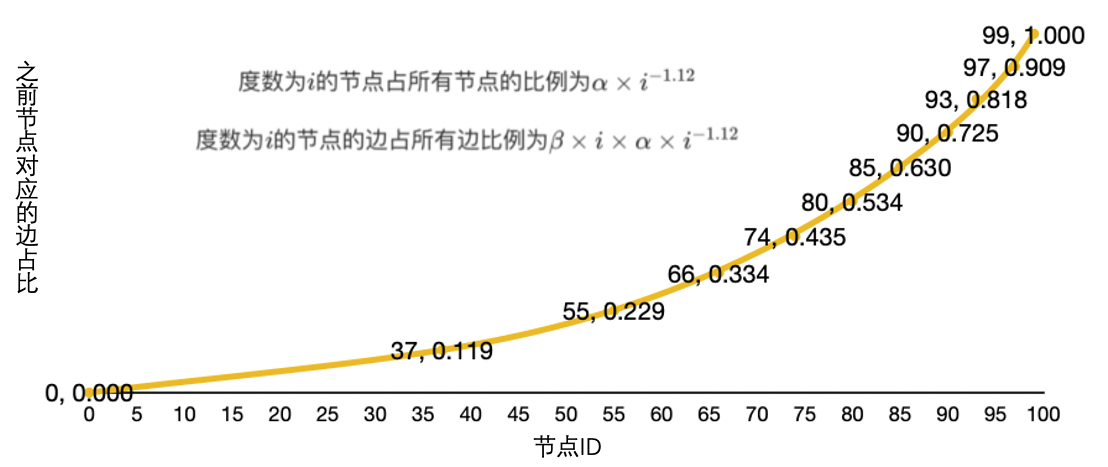
\includegraphics[scale=0.3]{choose_t1.png}
    \caption{示例-一个Power-Law分布节点选择过程1}
    \label{fig:target_node_choose1}
  \end{figure}
  
  如图\ref{fig:target_node_choose1}所示,图中标出的节点横纵坐标其实是累积量,如$55, 0.229$点表示入度不超过$2$的节点一共有$55$个,并且以这些节点为目标节点的边占比为$22.9\%$:
  
  \begin{itemize}
    \item 横坐标:入度不超过$m$的节点个数:$100 \times \sum\limits_{i = 1}^{i <= m} \alpha \times i^{-1.12}$
    \item 纵坐标:目标节点入度不超过$m$的边占比:$\sum\limits_{i = 1}^{i <= m} \beta \times i \times \alpha \times i^{-1.12}$
  \end{itemize}

\vspace{0.2cm}

  由于图中纵坐标表示的是边的累计分布。因此在选择目标节点时,可以在$[0, 1)$区间内得到一个随机数$r$,找到纵坐标为$r$对应点的横坐标,即为需要的节点序号。这一过程可以分为两步:确认入度范围、在范围中取值找到目标节点序号。

  \begin{figure}
    \centering
    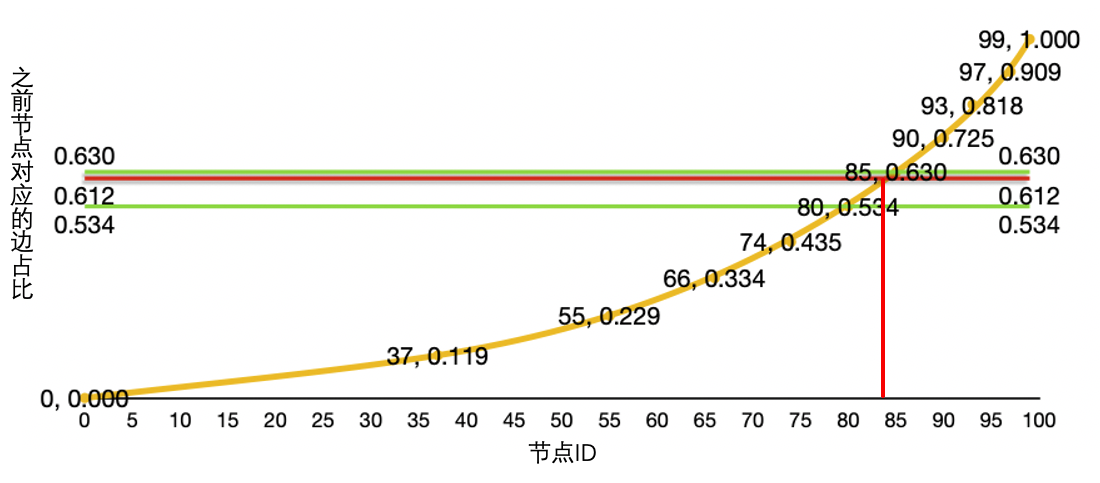
\includegraphics[scale=0.3]{choose_t2.png}
    \caption{示例-一个Power-Law分布节点选择过程2}
    \label{fig:target_node_choose2}
  \end{figure}
  
  如图\ref{fig:target_node_choose2}所示,当随机数选择为$0.612$时,确定横坐标的过程可以为:

  \begin{itemize}
    \item 确认$0.612$对应的点所在区间:从图\ref{fig:target_node_choose2}上可以看到$0.534<0.612<0.630$,两个定位点分别是$80, 0.534$和$85, 0.630$,所以应当在入度为$6$的节点中选择
    \item 目标节点序号取为:$80+\frac{0.612-0.534}{0.630-0.534} \times(85-80) \approx 84$
  \end{itemize}
\end{example}

通过对例\ref{exa:choose_t_graph}的讨论,可以得到目标节点选择算法的一个直观理解。接下来,将对例子中涉及到的公式进行重新定义,并且给出一个完整的选择算法。

% 但是上述算法存在一些问题:

% \begin{itemize}
%   \item 在给定随机数之后找到这个纵坐标对应的点需要用遍历或二分查找的方法,在度数范围比较大的情况下可能需要较长时间。
%   \item 节点个数变化时需要重新计算对应的横坐标。
% \end{itemize}

首先为所有节点分配一个重要性排序,排序在前的节点重要性较低即入度较小。

用公式\ref{equ:NodeInDegreeDetermine}即可确定每一个入度的节点在所有节点中占的比例,进而用累积的方法即可得到在节点排序中的区间。

\vspace{-8mm}

\begin{equation}
  \label{equ:NodeInDegreeDetermine}
  P\left(ind_i=m\right)=\frac{dist_{in}(m)}{\sum\limits_{j=d_{min}}^{d_{max}}dist_{in}(j)}
\end{equation}

确定一条边的目标节点时,需要按照公式\ref{equ:TargetProb}计算目标节点的入度为$m$的概率。

\vspace{-8mm}

\begin{equation}
  \label{equ:TargetProb}
  P\left(ind_{edge_i}=m\right)=\frac{dist_{in}(m) \times m}{\sum\limits_{j=d_{min}}^{d_{max}}dist_{in}(j)\times j}
\end{equation}

这里需要特别注意,在公式\ref{equ:NodeInDegreeDetermine}和公式\ref{equ:TargetProb}中,分别计算的是\textbf{所有节点中入度为i的概率}和\textbf{所有边中目标节点中入度为i的概率},因此其表示形式不同。

基于前述讨论,边的目标节点选择过程包含以下几步:

\begin{enumerate}
  \item 确定每个节点的排序信息,可以使用一个随机打乱函数实现;
  \item 依据公式\ref{equ:NodeInDegreeDetermine},按照排序信息给确定每个度数对应的节点范围,排序在前的节点入度较低;
  \item 依据公式\ref{equ:TargetProb},计算该边选择目标节点度数为$i$的概率$P$;
  \item 按照得到的概率$P$,随机选择每一条边目标节点对应的入度;
  \item 得到入度后,在这个入度对应的节点范围中进行随机选择。
\end{enumerate}

\vspace{0.2cm}

在例\ref{exa:choose_t}中给出了一个计算公式\ref{equ:NodeInDegreeDetermine}和公式\ref{equ:TargetProb}两个概率的示例。

\begin{example}
  \label{exa:choose_t}
  两个概率的计算\\
  \textbf{条件:}节点个数为2,入度范围为$[1,2]$,对应的概率密度函数为:$P(ind_i=1)=0.4, P(ind_i=2)=0.6$,节点排序为[1,0](即:下标为0的节点代表2号节点)\\
  \textbf{计算过程:}
  \begin{itemize}
    \item 所有节点中入度为1的概率为0.4,入度为2的概率为0.6
    \item 节点$[0, 0.8)$对应的入度分配为1,节点$[0.8,2]$的入度分配为2\footnote{注意这里的节点范围是浮点数而非整数。如果后续确定应该在入度为2的节点中选择,则会在$[0.8,2]$范围内均匀取随机数取整得到结果,即所得结果在$[0.8,1)$范围内则目标节点为排序中下标为0的节点。同时,也可以直接对每个入度对应的节点范围取整处理而非使用浮点数。}
    \item 选择的目标节点入度为1的节点的概率为$\frac {0.4\times 1}{0.4\times 1 + 0.6\times 2}=0.25$
    \item 选择的目标节点下标为0(2号)的概率为$0.25 + (1-0.25)\times\frac{1-0.8}{2-0.8}=0.375$
  \end{itemize}
\end{example}

进行目标节点选择的完整算法如算法\ref{alg:TargetNodeProb}所示。

\begin{algorithm}[htb]
  \caption{确定一条边的目标节点}
  \label{alg:TargetNodeProb}
  \begin{algorithmic}[1]
    \Require
      入度分布的概率密度函数$dist_{in}$,
      入度分布最小度数$d_{min}$,
      入度分布最大度数$d_{max}$,节点排序数组$Nodes$
    \Ensure 某条边的目标节点
    \Function {EdgeDegreeProb}{$dist_{in}, d_{min}, d_{max}$}
      \State $P \gets []$
      \State $sum \gets 0$
      \For{each $i\in [d_{min}, d_{max}]$}
        \State $P[i - d_{min}] \gets dist_{in}(i) \times i$
        \State $sum \gets sum + P[i - d_{min}]$
      \EndFor
      \For{each $i\in [d_{min}, d_{max}]$}
        \State $P[i - d_{min}] \gets P[i - d_{min}] / sum$
      \EndFor
      \State \Return $P$ // 每一个度数对应的概率$P$(列表形式,第一个元素对应于$d_{min}$)
    \EndFunction
    \State $P \gets$ DegreeProb$(dist_{in}, d_{min}, d_{max})$ // 可以直接调用确定出度概率的函数
    \State $P_{edge} \gets$ EdgeDegreeProb$(dist_{in}, d_{min}, d_{max})$
    \Function {GetTargetNode}{$d_{min}, d_{max}$}
      \State $degree \gets choice([d_{min}, d_{max}], P_{edge})$
      \State $node \gets choice(P[degree])$
      \State \Return $Nodes(int(node))$
    \EndFunction
  \end{algorithmic}
\end{algorithm}

\subsection{社区处理}
\label{cha:Community}

社区的划分其实就是将节点对应的ID进行分类,可以用一个字典结构对社区信息进行存储。实现时可以根据配置信息中指定的每个社区对应的规模,进行节点所属社区的随机分配。

在\ref{cap:simplegen}节中曾给出了社区参数$\rho$的定义,表示社区间生成边的概率与社区内部生成边的概率的比值。为了生成能够满足社区结构的图,可以对于生成的每一条边进行检测,得到的结果如果不在同一个社区内则按照概率$1-\rho$进行舍弃。这样得到的图即可满足社区参数$\rho$的要求。

\section{动态图事件处理}

第\ref{cha:staticgraph}节对生成静态图的方法进行了探讨,给出了对应的伪代码。而为了生成动态图,需要基于上述过程进行扩展,加入在第\ref{cha:chapter02}章讨论的动态特性。

在表\ref{tab:events}中已经定义了多种动态图事件,此处需要将这些事件进行具体的实现,分别是:

\begin{itemize}
  \item 节点个数的变化
  \item 边个数的变化
  \item 节点在分布中的重要度变化
  \item 社区参数的变化
\end{itemize}

\vspace{0.2cm}

在进行事件具体的实现之前,首先对需要记录的数据类型进行分析。除了节点、边、社区信息需要存储之外,节点在分布中的重要度信息也是必不可少的,\ref{cha:node_map}节中将对节点重要性的表征方式进行介绍。

\subsection{节点映射}
\label{cha:node_map}

在出度确定与边的目标节点确定过程中,都会体现出节点度数的不同,而这也就体现了不同节点的重要程度,并且在事件中也会有与节点重要度变化相关的内容。为了解决这一问题,本节提出了一种叫做“节点映射”的结构,用此结构进行节点重要度信息的存储。

节点映射包括两部分:

\begin{itemize}
  \item 出度分布:进行出度的分配后,得到的结果代表了节点的重要程度。因此,对于出度分布而言,可以直接使用初次分配得到的节点出度信息。
  \item 入度分布:第\ref{cha:DetermineTarget}节中曾经说明节点排序信息的重要性,入度分布节点映射即为对节点重要程度的表征。
\end{itemize}

\vspace{0.2cm}

形式上来说,节点映射的形式为:

\begin{itemize}
  \item 出度分布:节点ID到节点出度的字典。
  \item 入度分布:排序\footnote{排序在前的节点ID重要性较低,入度较小}后,节点ID组成的数组。
\end{itemize}

\vspace{0.2cm}

出度分布节点映射中的信息可以指导后续的生成过程。也就是说,对于初始重要度比较高(选定的出度更大)的节点,后续生成过程中的出度往往也会更大。入度分布节点映射则可以直接影响边目标节点的选择,在入度分布的节点映射不变的情况下,节点相对的重要程度在后续生成过程中也不会改变。

\subsection{事件的实现方式}

接下来,对各种事件的具体实现方式进行简要介绍。

由于事件中需要确定每个事件发生、结束的时刻,因此本节引入了“帧”的概念。一帧代表一个时刻,对应于动态图中保存的一个快照。同时,配置时需要提供动态图中涉及到的总帧数(动态图存储的快照数目,即时间序列的长度),以便在后续的生成过程中使用。

\subsubsection{边的生成}

在动态图的生成过程中,边的生成是里面非常重要的一部分。一种比较简单的生成方式是:

\begin{enumerate}
  \item 根据给定的节点配置、边的出度分布信息,计算出每一个节点的出度;
  \item 根据给定的帧数进行分配,计算得到该帧需要生成的边个数。这一过程中可以在平均分配的基础上加入随机因素;
  \item 根据得到的该帧边数目进行生成操作。
\end{enumerate}

\vspace{0.2cm}

\subsubsection{节点新增}

在新增节点后需要重新调整节点映射,其中的关键在于原有节点重要性信息的保持。

对于出度分布而言,在不改变原有节点出度的基础上计算新的节点出度即可。但是对于入度分布,需要考虑原有节点在所有节点中相对位置,可以用等比例缩放的方法。具体可以用式\ref{equ:newpos}表示,其中$N_{old}, N_{new}$分别表示新增节点前后的节点总数,$pos, pos_{new}$则分别表示新增节点前后的,某原始节点的位置(数组下标)。

\vspace{-8mm}

\begin{equation}
  \label{equ:newpos}
  pos_{new} = \text{int}\left(pos\times \frac{N_{new}}{N_{old}}\right)
\end{equation}

一种可行的实现方式为:

\begin{itemize}
  \item 出度分布节点映射:重新生成,为新节点分配出度。
  \item 入度分布节点映射:将原有节点的位置等比例缩放,剩余的空间随机填入新增的节点。\\
  例如,原有节点一共有3个,入度分布节点映射为$[1,2,0]$。在新增7个节点之后,原有节点ID调整到了如下位置:$[1,\_,\_,2,\_,\_,0,\_,\_,\_]$,空余位置会将新节点调整顺序之后排入。
\end{itemize}

\vspace{0.2cm}

除此之外,还需要考虑新节点所属社区。在此可以采用随机的方式,根据不同社区的规模按照对应比例进行社区分配。

\subsubsection{边与节点删除}

边的删除较为简单,直接从记录中按照要求去掉对应比例边即可。节点删除会导致其关联的边删除,并且节点映射等结构也会随之受到影响。

对于节点的删除事件,在一些真实社交网络上并不多(相对于节点新增而言),如在微博上关注关系图中用户被官方封号、引文网络某篇文章被撤稿,在这两个社交网络中节点删除的操作并不多。

为了尽量减少总的运算量,可以采用集合的方式记录被删除的节点,在新的生成过程中遇到这个节点后跳过即可。

在实现过程中可以设置一个阈值$\alpha$,若删除节点数与总节点数的比值低于$\alpha$则使用前述集合记录被删除节点的方式,反之则进行节点映射的调整,具体操作同节点新增操作。

\subsubsection{社区结构变化}

在日常生活中经常可以看到不同社区之间融合、小团体的形成等现象,这些对应于社区结构的变化。这些变化特征包括社区参数$\rho$的变化与社区的融合、分裂操作。

在\ref{cha:Community}节中介绍了社区的应用方式,社区结构可以用一个字典形式进行存储,对社区结构的改变与参数$\rho$的改变只作用于后续新生成的边,新生成的边按照新的社区划分与参数$\rho$进行一定概率的舍弃操作即可。

\subsubsection{节点重要度改变}

在表\ref{tab:events}中,定义了两个与节点重要度改变有关的事件,分别是“突发事件”与“节点重要度变化”,前者是聚焦于突发事件导致的节点重要度的临时性改变,而后者则着重强调节点重要度的永久性改变。临时性改变是可逆的,因此需要保存改变的记录,以便后续恢复。

在节点重要度变化的过程中,修改的其实就是分布对应的节点映射。因此,需要分出度分布和入度分布分别讨论:

\begin{itemize}
  \item 出度分布节点映射:可以将其中某个节点的出度提高,或者将两个节点的出度互换;
  \item 入度分布节点映射:将两个节点的位置互换即可。
\end{itemize}

\vspace{0.2cm}

\section{可配置动态图生成组件的实现}
\label{cha:tool_implementation}

在前两节进行了动态图生成算法的介绍,具体实现时则较为复杂,还考虑配置解析、整体架构、存储方式等内容,在此节中将会对这些内容进行介绍。

\subsection{整体架构}

生成组件时的整体架构如图\ref{fig:structure}所示,具体介绍如表\ref{tab:dyn_stru}所示。

\begin{table}[htb]
  \centering
  \caption[动态社交网络图生成整体架构]{动态社交网络图生成整体架构}
  \label{tab:dyn_stru}
  \begin{minipage}[t]{1\textwidth}
    \begin{tabularx}{\linewidth}{llX}
      \toprule[1.5pt]
      {\heiti 层级} & {\heiti 名称} & {\heiti 说明} \\
      \midrule[1pt]
      解析层 & 配置解析器 & 相关配置的输入与解析 \\\hline
      调度层 & 调度管理器 & 接收解析部分得到的配置信息,进行任务安排、相关内容的存储 \\\cline{2-3}
       & 事件列表 & 解析与存储用户定义的各类事件 \\\cline{2-3}
       & 任务列表 & 将图的生成与各种事件抽象为“任务”这一概念,每一个任务可能由几个步骤组成 \\\cline{2-3}
       & 行为列表 & 将任务进行后续处理,其中对结构有影响的基本步骤被称为“行为”(如:修改某个边对应分布的节点映射,修改某个边对应社区的参数) \\\cline{2-3}
       & 节点信息 & 节点标签、数量、属性,事件中被删除、禁用的节点列表等 \\\cline{2-3}
       & 边信息 & 边的标签、属性、社区配置、分布信息、节点映射等 \\\cline{2-3}
       & 存储信息 & 存储格式、所在目录等 \\\hline
      生成层 & 事件执行器 & 根据指令执行各事件对应的行为,可能修改动态图结构特征 \\\cline{2-3}
       & 生成管理器 & 调用事件执行器进行相应事件的执行,并且进行生成操作,将每一帧生成的结果送入存储管理器中保存 \\\cline{2-3}
       & 存储管理器 & 以指定格式在指定位置存储生成结果 \\
      \bottomrule[1.5pt]
    \end{tabularx}
  \end{minipage}
\end{table}

% \begin{itemize}
%   \item 解析部分:相关配置的输入与解析,进行调度与生成工具的配置与初始化;
%   \item 调度与生成工具部分:接收解析部分得到的配置信息,进行任务安排、相关内容的存储,包含以下部分:
%   \begin{itemize}
%     \item 任务列表生成:将图的生成与各种事件抽象为“任务”这一概念,每一个任务可能由几个步骤组成;
%     \item 行为列表生成:将之前得到的任务进行后续处理,其中对结构影响的基本步骤被称为“行为”(如:修改某个边对应分布的节点映射,修改某个边对应社区的参数);
%     \item 调度器:维护一个时钟,每一帧都检查该帧需要执行的基本步骤(即上文的“行为”),进行对应函数的调用;
%     \item 结构信息存储:存储在生成过程中需要的各种信息,包括:
%     \begin{itemize}
%       \item 节点标签、数量、属性,事件中被删除、禁用的节点列表等;
%       \item 存储相关的文件句柄、目录管理、已生成边和节点的记录等;
%       \item 边的标签、属性、社区配置、分布配置、节点映射等。
%     \end{itemize}
%   \end{itemize}
% \end{itemize}

\begin{figure}
  \centering
  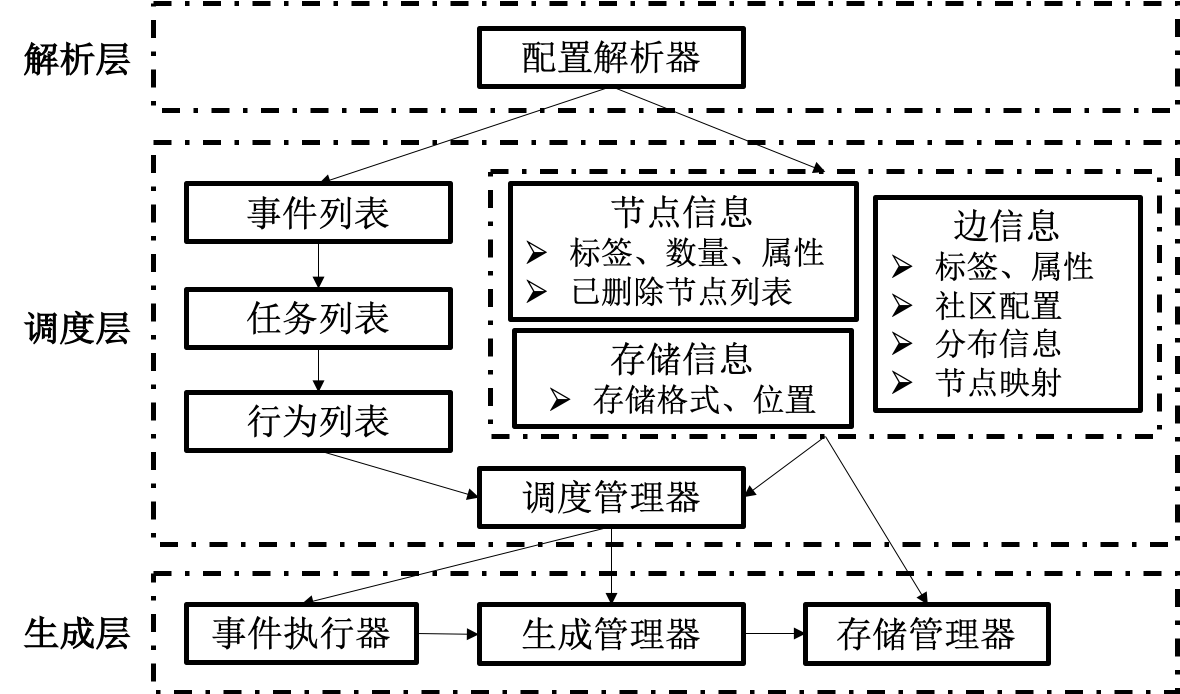
\includegraphics[scale=0.6]{structure_new.png}
  \caption{动态社交网络图生成整体架构}
  \label{fig:structure}
\end{figure}

解析层负责进行配置解析,用户自定义的配置信息在第\ref{cha:generatorscheme}节中有详细介绍,格式如表\ref{tab:dynamic_define}所示,主要包括节点、边、社区、事件这几部分内容,还可以指定存储格式与位置。通过这些信息,可以调度层中所示的事件列表、节点、边、存储的信息这些内容。其中事件列表会进行后续解析,得到每一个事件对应的任务,进一步拆解成一些行为序列(行为是指对结构有影响的基本的操作单元,如修改某个边对应社区的参数,一个任务中可能包括多个行为)。

接下来将由调度管理器进行管理,每一帧都调用对应的生成任务并进行事件的执行,每一帧的结果会送入存储管理器以给定格式在给定位置进行存储。

\subsection{结果保存}

\begin{table}[htb]
  \centering
  \caption[图存储结构]{生成的动态图存储结构}
  \label{tab:store}
  \begin{minipage}[t]{1\textwidth}
    \begin{tabularx}{\linewidth}{llXX}
      \toprule[1.5pt]
      {\heiti 分类} & {\heiti 名称} & {\heiti 说明} & {\heiti 示例(之前已有$0\rightarrow 1$,此帧新增$0\rightarrow 2, 1\rightarrow 2, 2\rightarrow 0$)} \\
      \midrule[1pt]
      快照形式$^{*}$ & TSV & 文本格式,每行记录一条边 & \tabincell{l}{0 1\\0 2\\1 2\\2 0} \\\cline{2-4}
       & ADJ & 文本格式,每行记录起始节点与对应的边 & \tabincell{l}{0 1 2\\1 2\\2 0} \\\cline{2-4}
       & CSR & 正向表,第一个文件记录节点后继的位置,第二个文件记录所有后继节点 & \tabincell{l}{第一个文件:0 2 3\\第二个文件:1 2 2 0} \\\cline{2-4}
       & Neo4j & 在Neo4j数据库中进行存储,以属性形式存储帧数信息,可以限定帧数进行查询 & 略 \\\cline{2-4}
       & node\_link & JSON格式存储、记录每一个节点、每一条边的信息 & \tabincell{l}{\{``directed": True,\\\ \ ``multigraph": False,\\\ \ ``graph": \{\},\\\ \ ``nodes": [\{``id": 0\},\\\ \ \ \ \{``id": 1\}, \{``id": 2\}],\\\ \ ``links": [\\\ \ \ \ \{``source": 0, ``target": 1\},\\\ \ \ \ \{``source": 0, ``target": 2\},\\\ \ \ \ \{``source": 1, ``target": 2\},\\\ \ \ \ \{``source": 2, ``target": 0\}]\}} \\\hline
      增量形式 & DIFF & JSON格式存储增加与删除的边、增加与删除的节点 & \tabincell{l}{\{``nodes\_added": [2],\\\ \ ``nodes\_deleted": [],\\\ \ ``edges\_added": [(0, 2), \\\ \ \ \ (1, 2), (2, 0)],\\\ \ ``edges\_deleted": []\}}\\
      \bottomrule[1.5pt]
    \end{tabularx}\\[2pt]
    \footnotesize *:直接将每一帧的数据保存到一个文件中,以文件命名区分帧数
  \end{minipage}
\end{table}

本节将介绍动态图生成组件实现的一部分可用存储结构,并且用示例加以说明,具体如表\ref{tab:store}所示。

表\ref{tab:store}中所有列出的格式可以分成快照形式(每一帧的数据单独存储)与增量形式(记录每一帧与之前一帧的区别,以达到节省存储空间的目的)两类,其中增量形式所记录的新增的边、删除的边等内容也可以用与快照形式中相同的方法存储。

除了表\ref{tab:store}中呈现的格式,还实现了networkx中支持的GraphML、ADJACENCY、CYTOSCAPE、JIT等格式,并且可以很方便地修改支持其他格式。

% !TeX root = ../main.tex

\chapter{动态社交网络图生成管理系统}
\label{cha:chapter04}

在第\ref{cha:chapter03}章中已经对生成算法与生成模块的具体实现方式进行了介绍,在本章中将设计并构建一个完整的动态社交网络图生成管理系统。

本系统使用网页配置的形式,可以让用户更方便地进行配置与修改,避免手写JSON等配置文件的不便。系统中使用Vue.js进行前端整个体系的搭建,其中用ElementUI进行美化,用Echarts进行相关可视化的操作;并且使用Django进行后端Restful API的搭建,将第\ref{cha:chapter03}章中实现的可配置动态社交网络图生成算法作为其中的一个组件接入,以便用户方便、直观地进行系统的使用。

接下来将从管理系统的整体系统架构、执行流程的方面进行介绍。

\section{系统架构}

\begin{figure}[H]
  \centering
  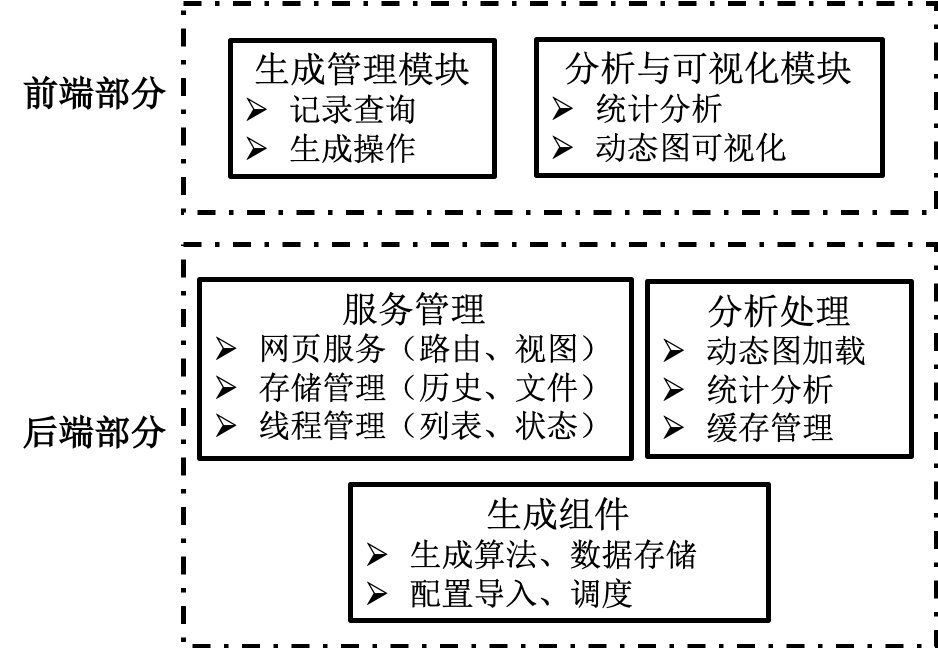
\includegraphics[scale=0.6]{structure_system_new.png}
  \caption{动态社交网络图生成管理系统整体架构}
  \label{fig:web_system}
\end{figure}

如图\ref{fig:web_system}所示,系统使用前后端分离的Restful架构设计,在后端Django服务中接入第\ref{cha:chapter03}章中实现的可配置动态图生成算法作为其中的生成组件。

前端的生成管理模块负责用户在网页上查询历史生成记录、填写配置信息并进行生成操作,分析与可视化模块为用户展示各项统计分析的图表与可视化的图数据。前端部分主要的工作集中于图的配置、生成与后续的分析、可视化操作。其中图的生成命令、生成结果与历史记录、分析数据的获取都用网络请求API与后端进行交互。

后端部分相对较为复杂,关键点在于将生成组件与网页服务结合在一起。

后端的服务管理模块包括Django服务本体与我自己编写的存储管理、线程管理两部分内容。

由于需要进行大量的生成与结果查询的工作,在后端服务中设计实现了用于结果存储的模块。使用数据库进行配置信息、生成记录、文件存放位置、线程状态等内容的存储。

由于生成过程时间较长会阻塞网页请求,因此在系统中使用了多线程的方法,配置了一个专门的线程管理器,每次有生成请求时便分配给一个新的线程,结果查询时会检测线程是否成功结束。这样的设计也可以很好地避免生成组件部分出现问题导致进程挂起,提高了整个系统的可靠性。

后端的分析处理模块用于处理前端的统计分析、可视化需求,在后端计算得到展示用的数据后返回给前端。并且为了为了节省带宽、加快访问速度,避免不必要的计算,设计了缓存机制。

而后端的生成组件就是第\ref{cha:chapter03}章中对生成算法的实现,并且为了与后端互动集成了配置导入与生成调度部分。

主页设计如图\ref{fig:frontend-home}所示,展示了所有的生成记录,并且使用不同颜色代表不同生成状态。在此页面中用户可以选择某一个记录进行后续的分析与可视化操作。

\begin{figure}[H]
  \centering
  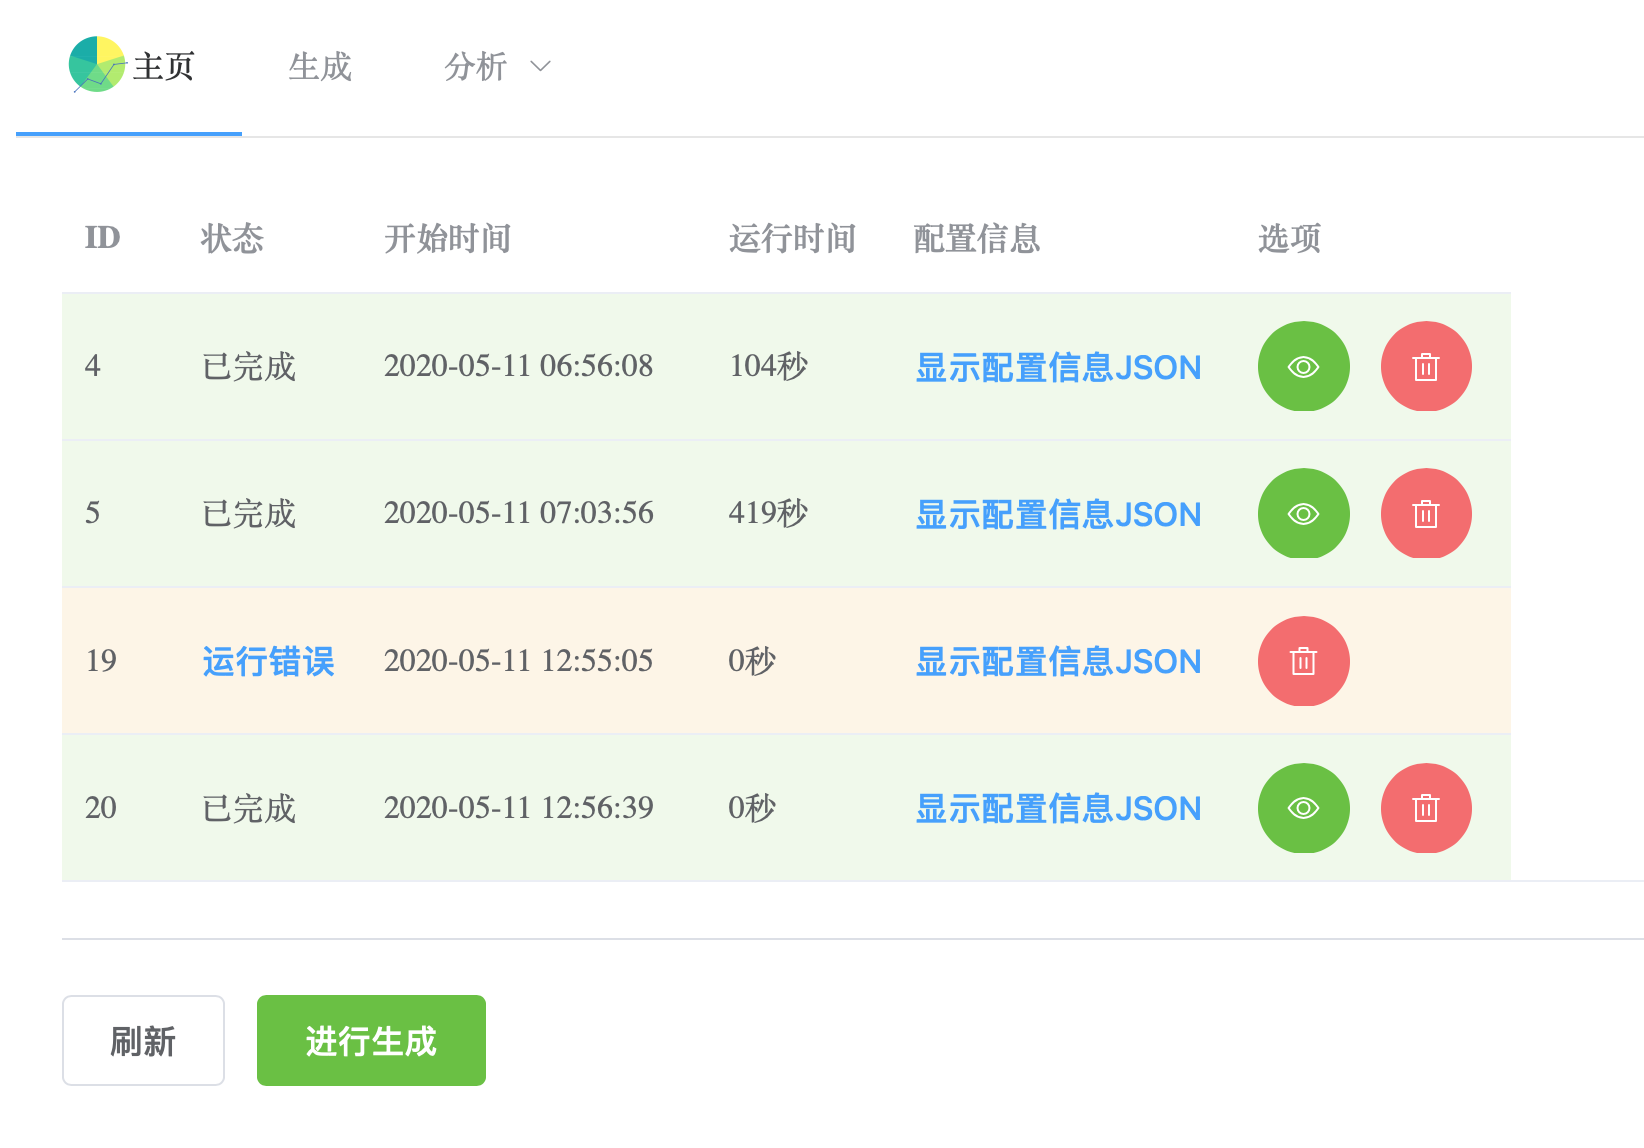
\includegraphics[scale=0.4]{frontend-home.png}
  \caption{管理系统-主页设计}
  \label{fig:frontend-home}
\end{figure}

在配置选择页面,用户可以用交互式操作进行每一个选项的详细配置。如图\ref{fig:iterations_node}、\ref{fig:edge_comm_event}所示。

\begin{figure}[H]
  \centering
  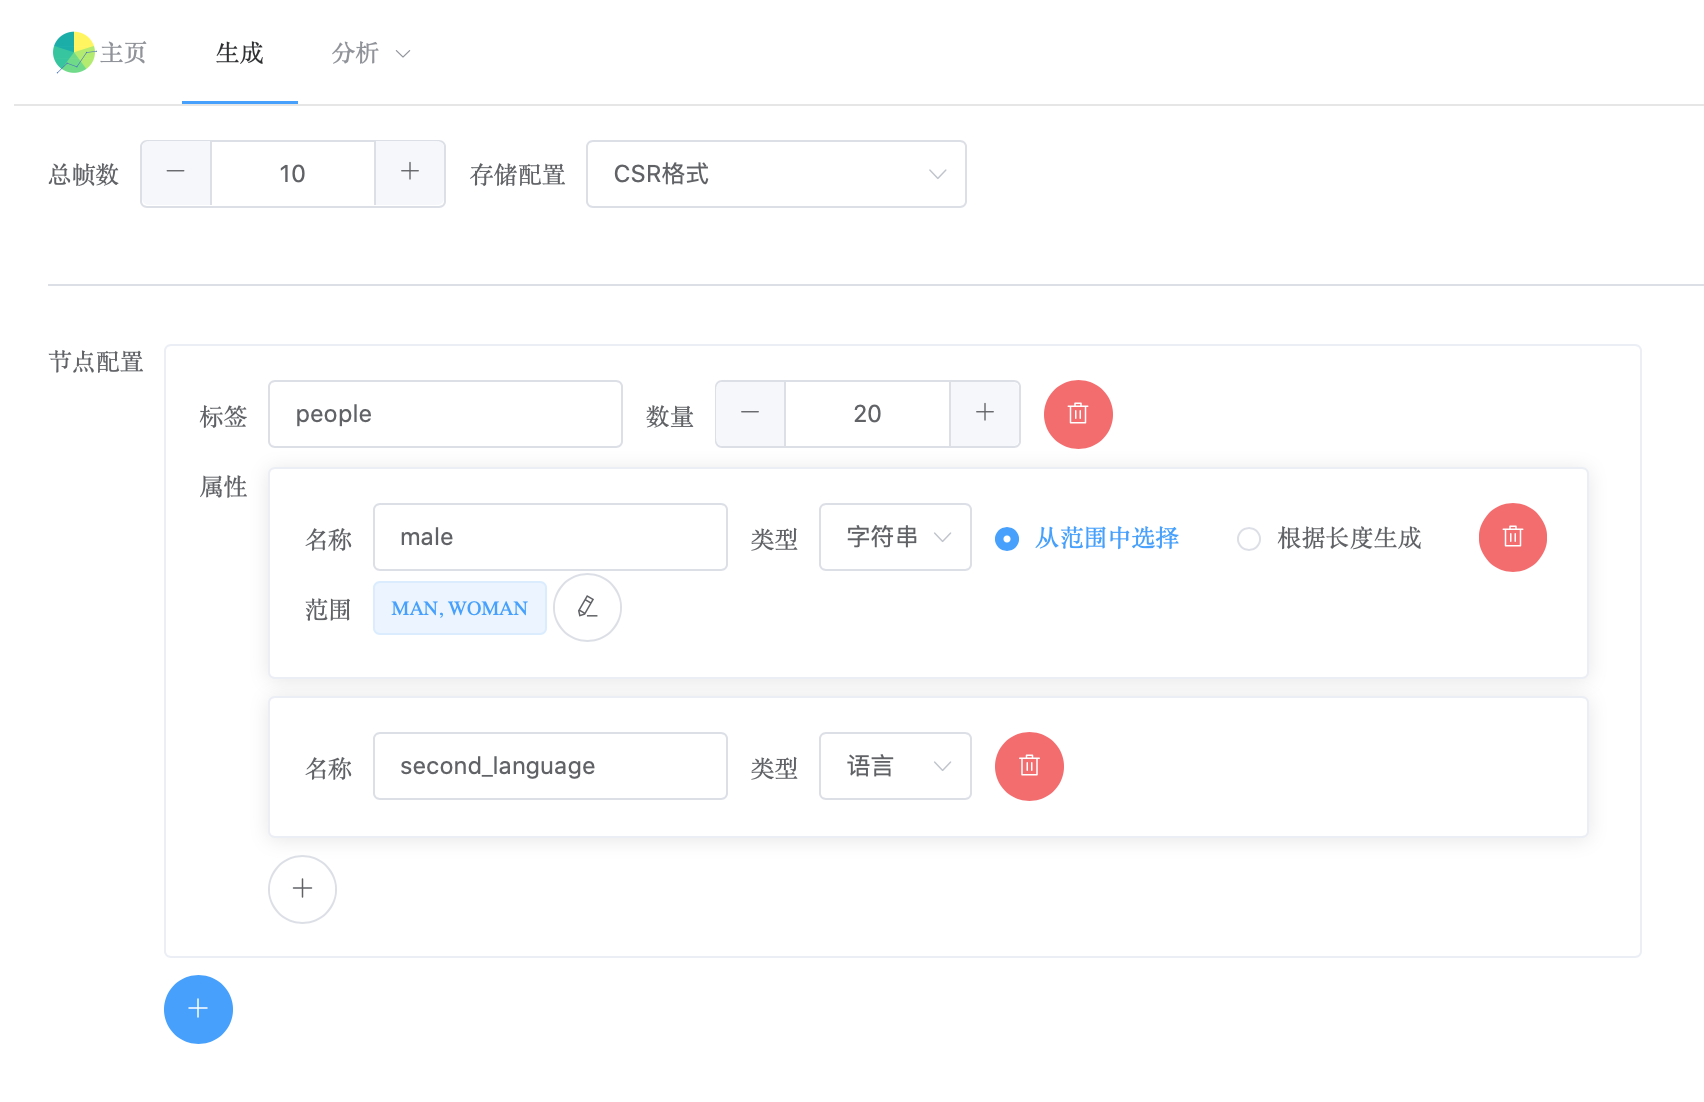
\includegraphics[scale=0.4]{iterations_node.png}
  \caption{管理系统-生成配置选项1}
  \label{fig:iterations_node}
\end{figure}

\begin{figure}[H]
  \centering
  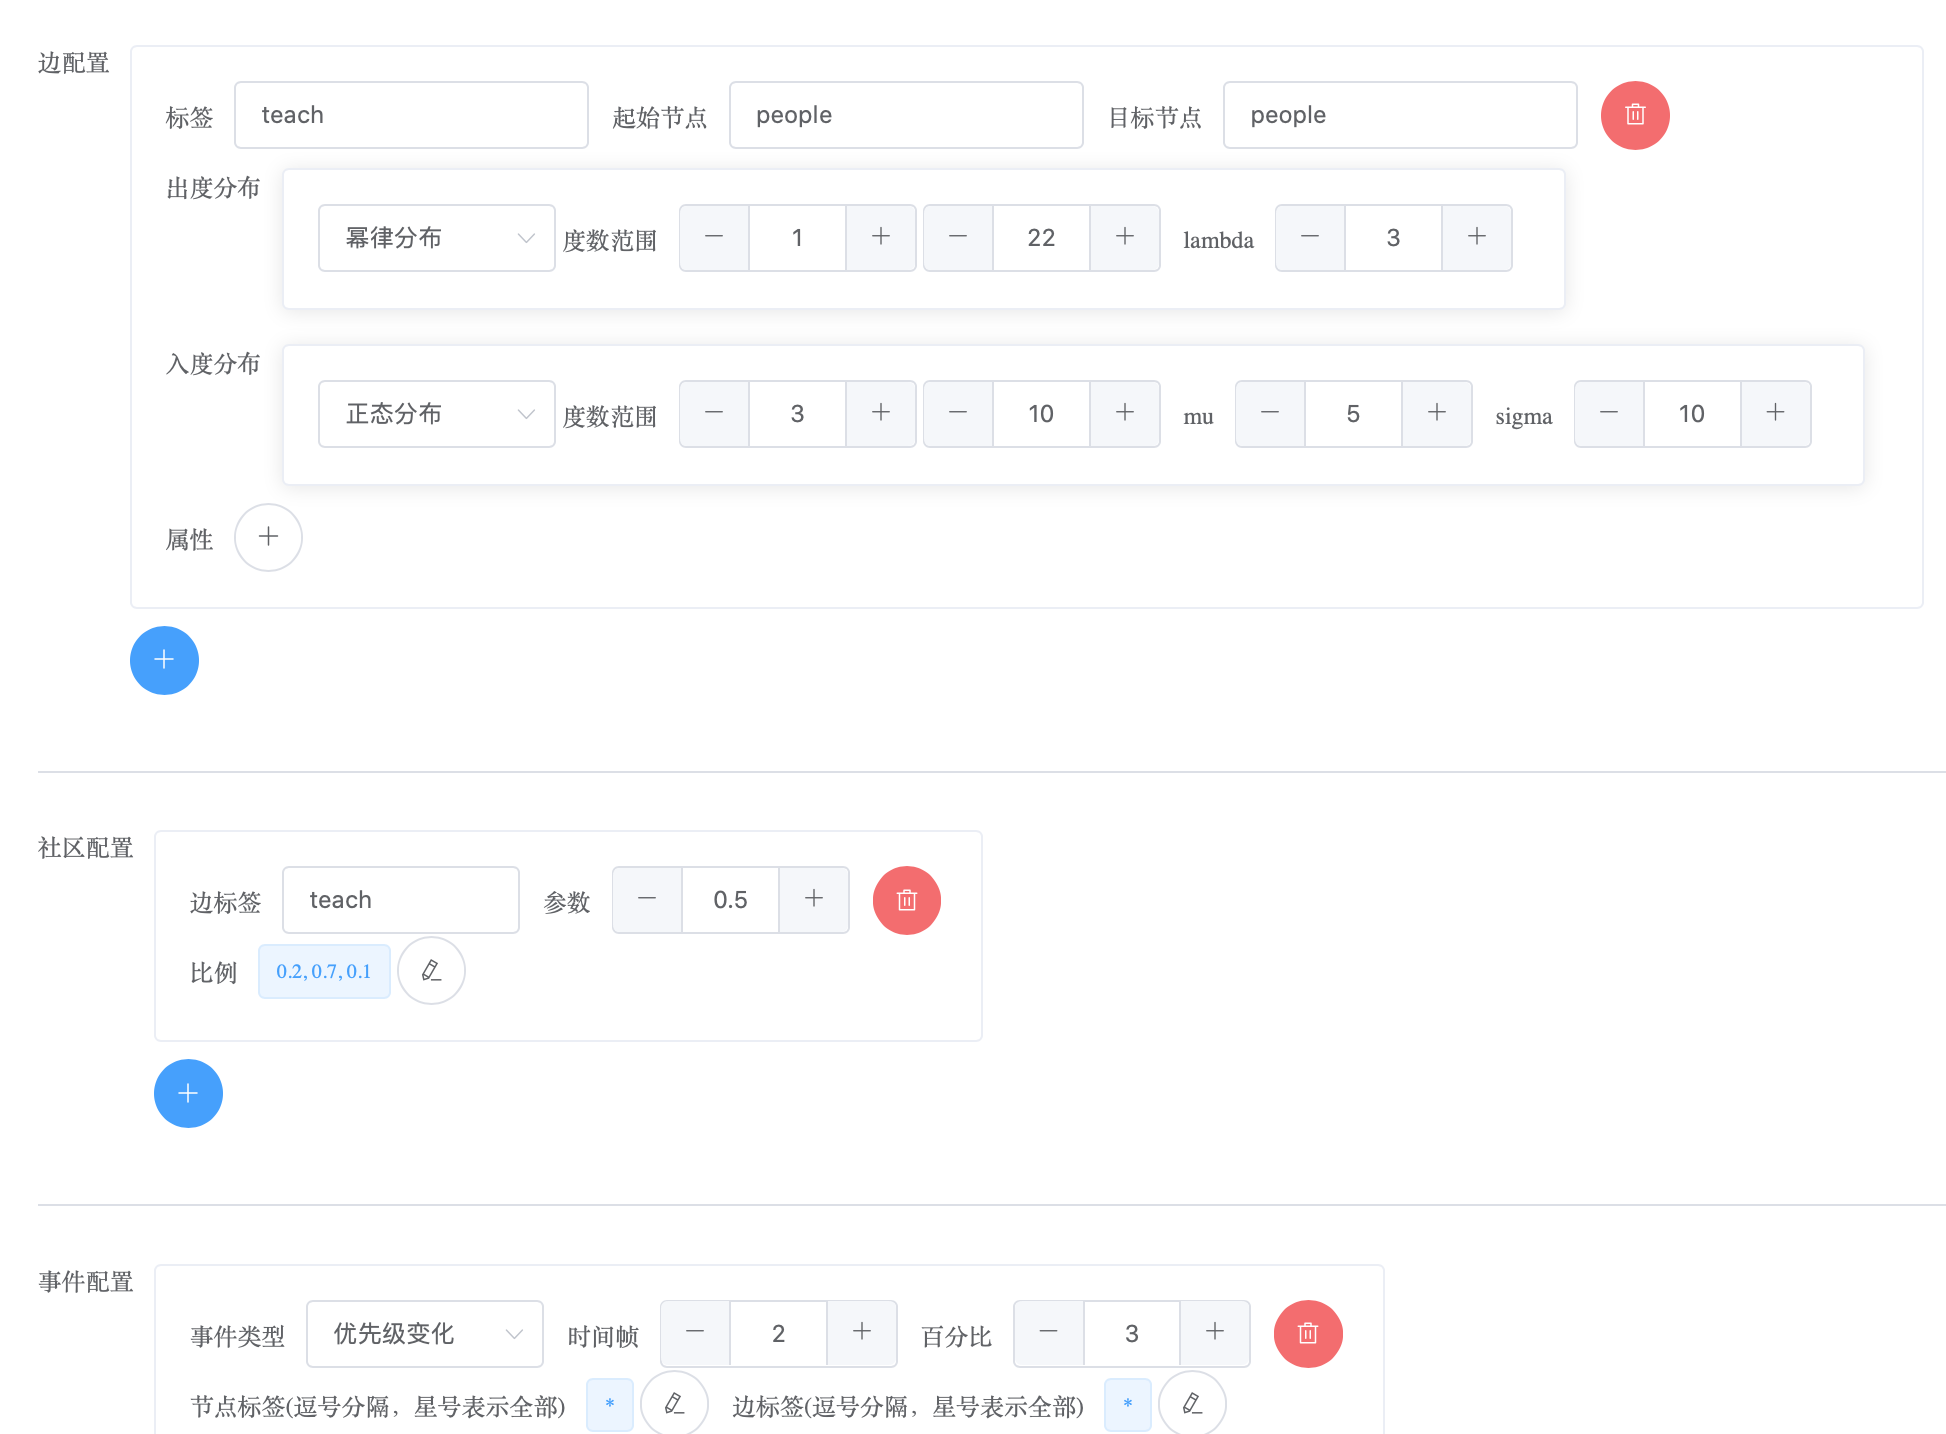
\includegraphics[scale=0.4]{edge_comm_event.png}
  \caption{管理系统-生成配置选项2}
  \label{fig:edge_comm_event}
\end{figure}

如图\ref{fig:analyzepage}所示,系统中实现了如下几种分析与可视化的显示:度数分布\footnote{度数分布部分展示每一个时刻对应的度数分布图}、度数变化\footnote{度数变化部分在选定一个节点,进行该节点度数变化分析}、节点变化\footnote{节点变化部分展示在各个事件中影响了哪些节点}、图可视化\footnote{图可视化部分会逐帧展示每一个时刻的图}。

\begin{figure}[H]
  \centering
  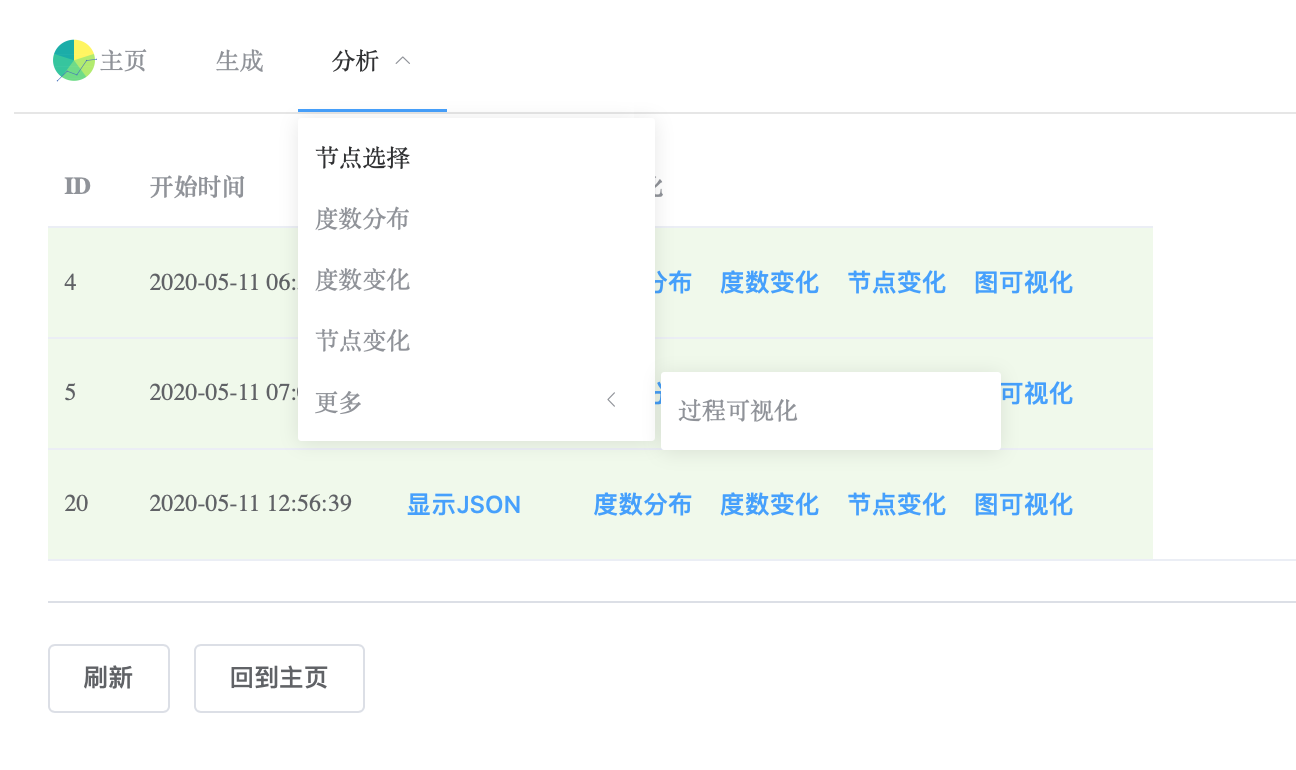
\includegraphics[scale=0.5]{analyzepage.png}
  \caption{管理系统-分析选项}
  \label{fig:analyzepage}
\end{figure}

以度数分布为例,其显示结果如图\ref{fig:degree_show}所示。选择边的标签、时刻信息、出度/入度分布之后,即可看到在这一个时刻的分布特征。

\begin{figure}[H]
  \centering
  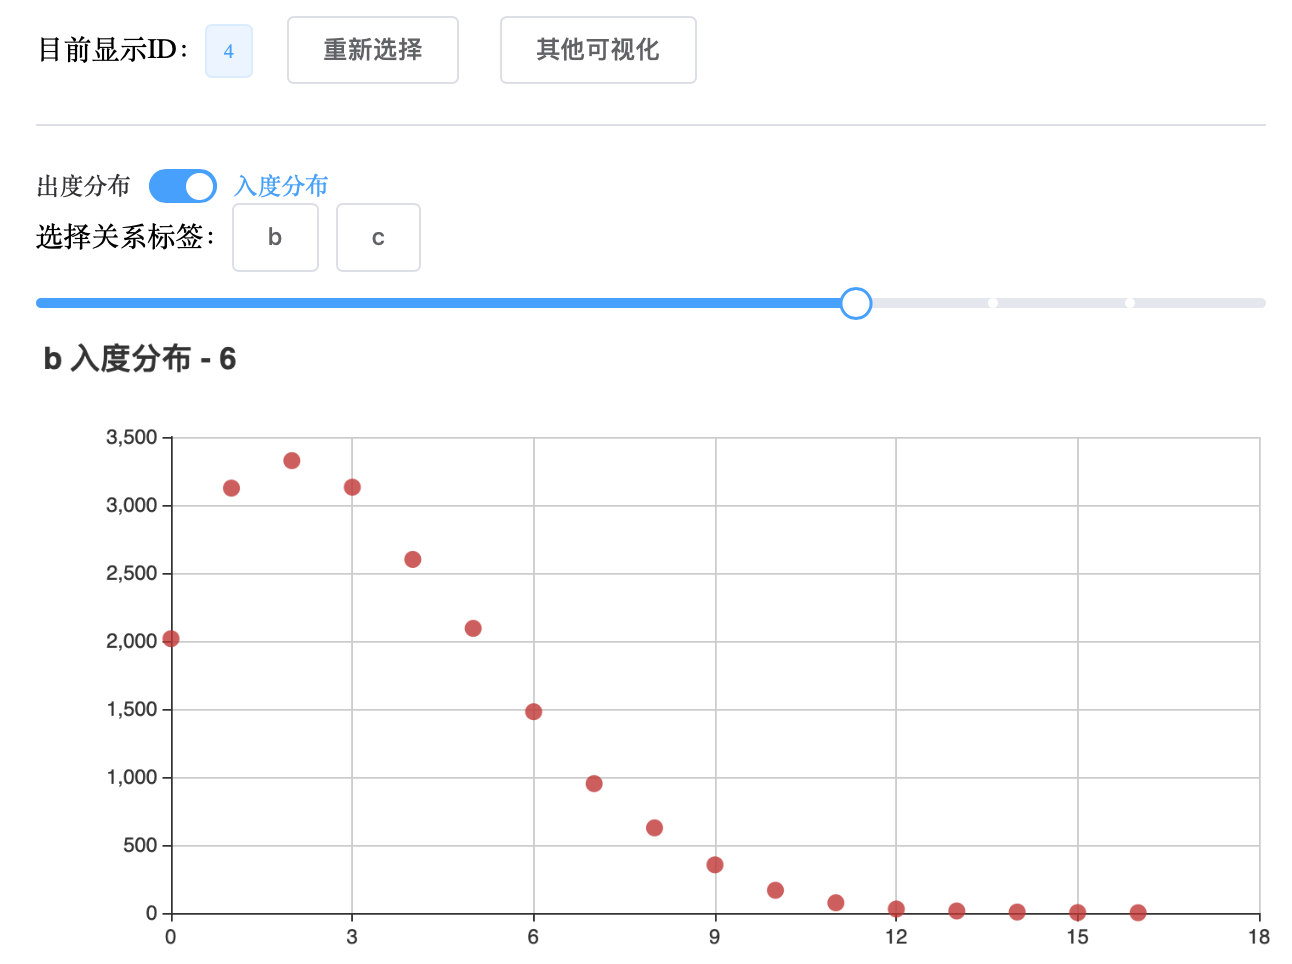
\includegraphics[scale=0.45]{degree_show.png}
  \caption{管理系统-度数分布分析}
  \label{fig:degree_show}
\end{figure}

\section{执行流程}

% 一个用户的典型操作过程与相应的前后端行为如下:

% \begin{enumerate}
%   \item 用户进入配置选择页面,进行所需动态图相关属性的配置(如图\ref{fig:iterations_node}、\ref{fig:edge_comm_event});
%   \item 前端将用户填写的配置信息转换为JSON格式,发送到后端;
%   \item 后端收到动态图生成请求与配置信息,分配一个新的线程进行生成操作,该线程会将生成任务相关信息存储到数据库中;
%   \item 用户获取生成结果,后端收到请求后在数据库中进行查询,若生成线程执行完成则将结果返回给前端进行结果的渲染与显示;
%   \item 用户选择进行可视化分析,后端收到请求后进行统计分析,将对应的结果返回前端进行渲染与展示。
% \end{enumerate}

% 具体执行流程如如图\ref{fig:stream}所示。

% \begin{figure}[H]
%   \centering
%   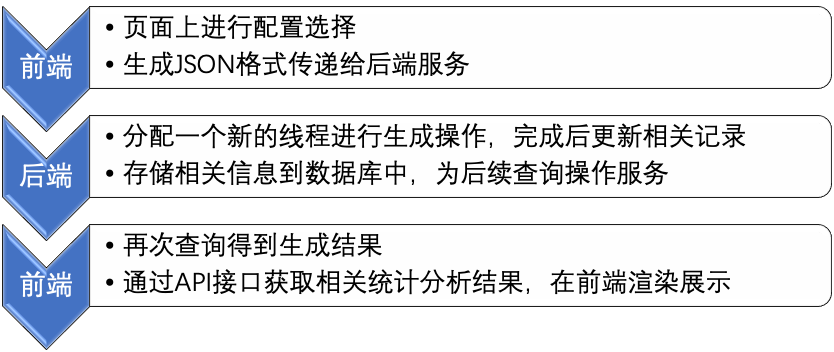
\includegraphics[scale=0.45]{stream.png}
%   \caption{管理系统-执行流程}
%   \label{fig:stream}
% \end{figure}

系统的具体执行流程如如图\ref{fig:uml_generate}与图\ref{fig:uml_analyze}所示。

\begin{figure}[H]
  \centering
  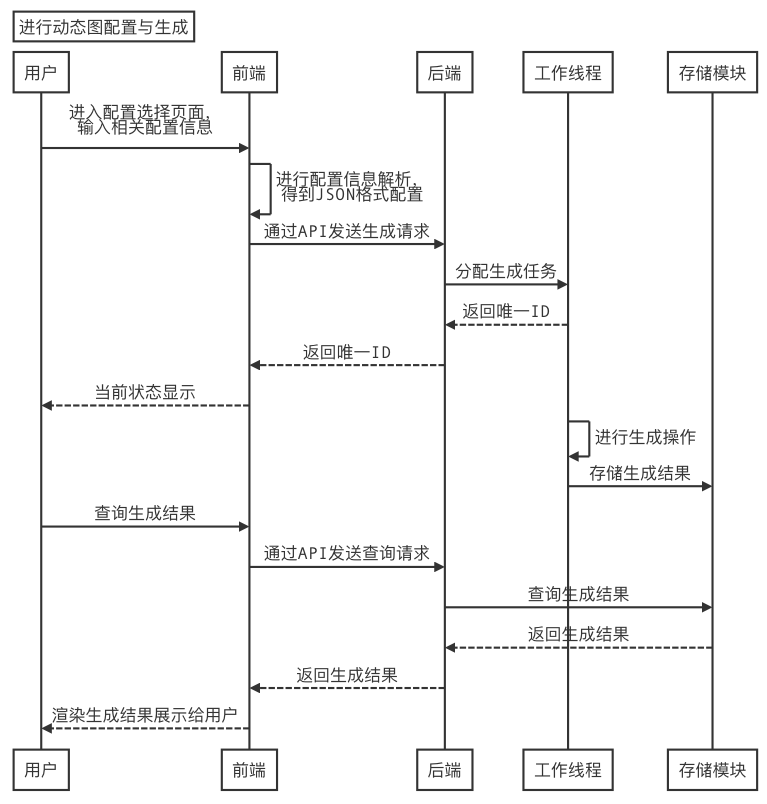
\includegraphics[scale=0.45]{uml_generate.png}
  \caption{动态图生成过程流程图}
  \label{fig:uml_generate}
\end{figure}

\begin{figure}[H]
  \centering
  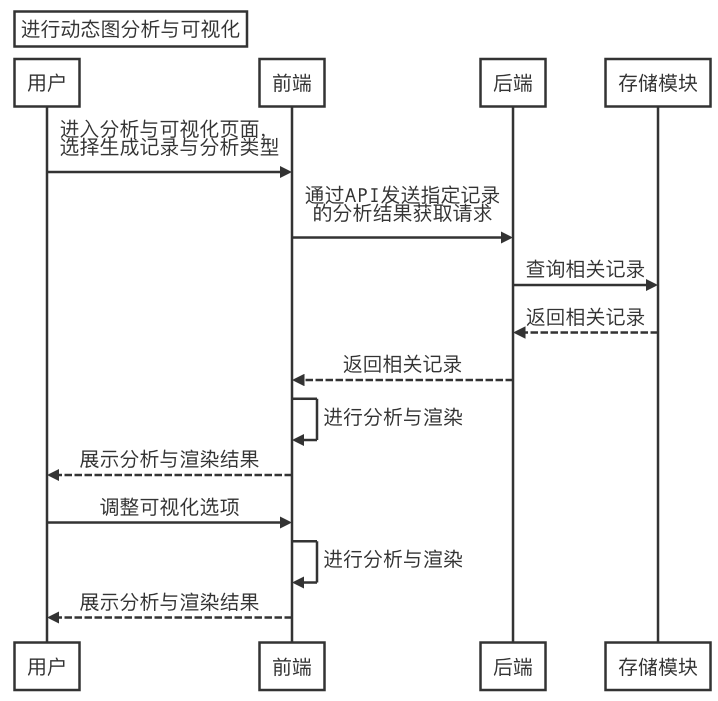
\includegraphics[scale=0.45]{uml_analyze.png}
  \caption{动态图分析与可视化流程图}
  \label{fig:uml_analyze}
\end{figure}
% !TeX root = ../main.tex

\chapter{实验}
\label{cha:chapter05}

本章将使用前文设计并实现的动态社交网络图生成系统进行实验,检验动态社交网络图生成算法所产生结果的各项性质并展示生成过程的复杂度。

实验过程中使用的机器配置如下:

\begin{itemize}
  \item 处理器:2.7 GHz 双核Intel Core i5
  \item 内存:8 GB 1867 MHz DDR3
  \item 系统:macOS 10.15.3
\end{itemize}

\section{动态图特征分析}

本节将使用指定的配置信息进行动态图的生成,并且检测生成的图是否满足要求。

本节使用如下配置方式,检验入度分布与出度分布是否符合预期:

\begin{itemize}
  \item 总帧数为$10$
  \item 定义了标签为student的节点、标签为friend的边,节点总数为$2000$,不存在多重边
  \item 入度分布与出度分布为$\lambda=2$的Power-Law分布
  \item 社区按照$8:2$的比例进行划分,社区参数$\rho=0.5$
  \item 定义以下事件:
  \begin{itemize}
    \item 第3帧:节点重要度变化,影响$1\%$的节点
    \item 第5-7帧:突发事件导致$1\%$节点重要度上升
    \item 第6帧:社区更为明显,社区参数变化为$\rho=0.3$
    \item 第5帧:节点增加,新增$50$个节点
    \item 第9帧:节点删除,原有的$90$个节点被删除
  \end{itemize}
\end{itemize}

由于Power-Law分布的概率密度函数为指数形式,因此将入度分布与出度分布使用对数坐标轴呈现,度数范围为$[1, 100]$的结果如图\ref{fig:parallel1}与图\ref{fig:parallel2}所示。

\begin{figure}
\begin{minipage}{0.48\textwidth}
  \centering
  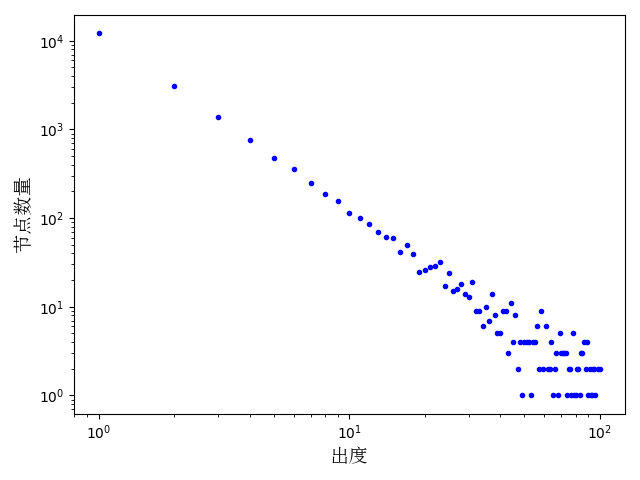
\includegraphics[scale=0.3]{out_degree_exp1.png}
  \caption{生成结果出度分布}
  \label{fig:parallel1}
\end{minipage}\hfill
\begin{minipage}{0.48\textwidth}
  \centering
  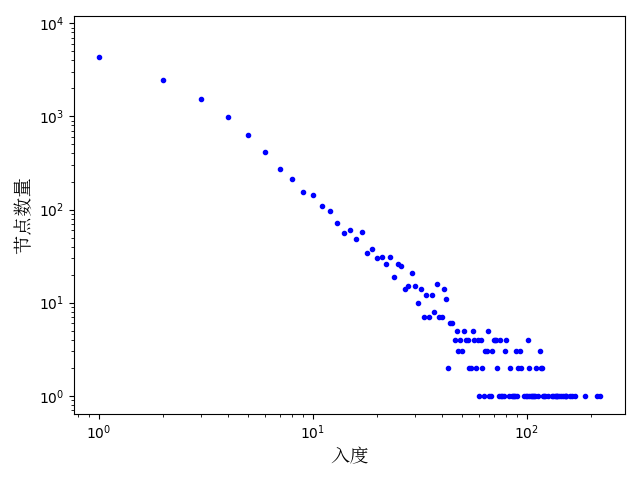
\includegraphics[scale=0.3]{in_degree_exp1.png}
  \caption{生成结果入度分布}
  \label{fig:parallel2}
\end{minipage}
\end{figure}

从图中可以看出,结果的出度分布范围与给定条件几乎完全吻合,从图上来看的确符合Power-Law分布。

总体来看,入度分布的确符合Power-Law分布。但入度分布与给定的条件并不完全相符,出现了许多度数超出配置时的度数范围($[1, 100]$)的节点。这是因为入度分布的信息只是提供目标节点选择概率的参考,由于入度分布于出度分布可能不相吻合,因此不会保证结果的入度分布完全符合给定的要求。

接下来检验单个节点的度数变化。为了避免度数极小的点对分析造成干扰,在此将度数范围设置为$[30, 100]$。

在此选择一些在事件中重要度发生变化的节点。如图\ref{fig:important_eg1}与图\ref{fig:important_eg2}所示,节点1514和节点326是节点重要度变化事件中受到影响的节点,其重要性分别在第3帧时得到提升与降低。

\begin{figure}[H]
  \centering
  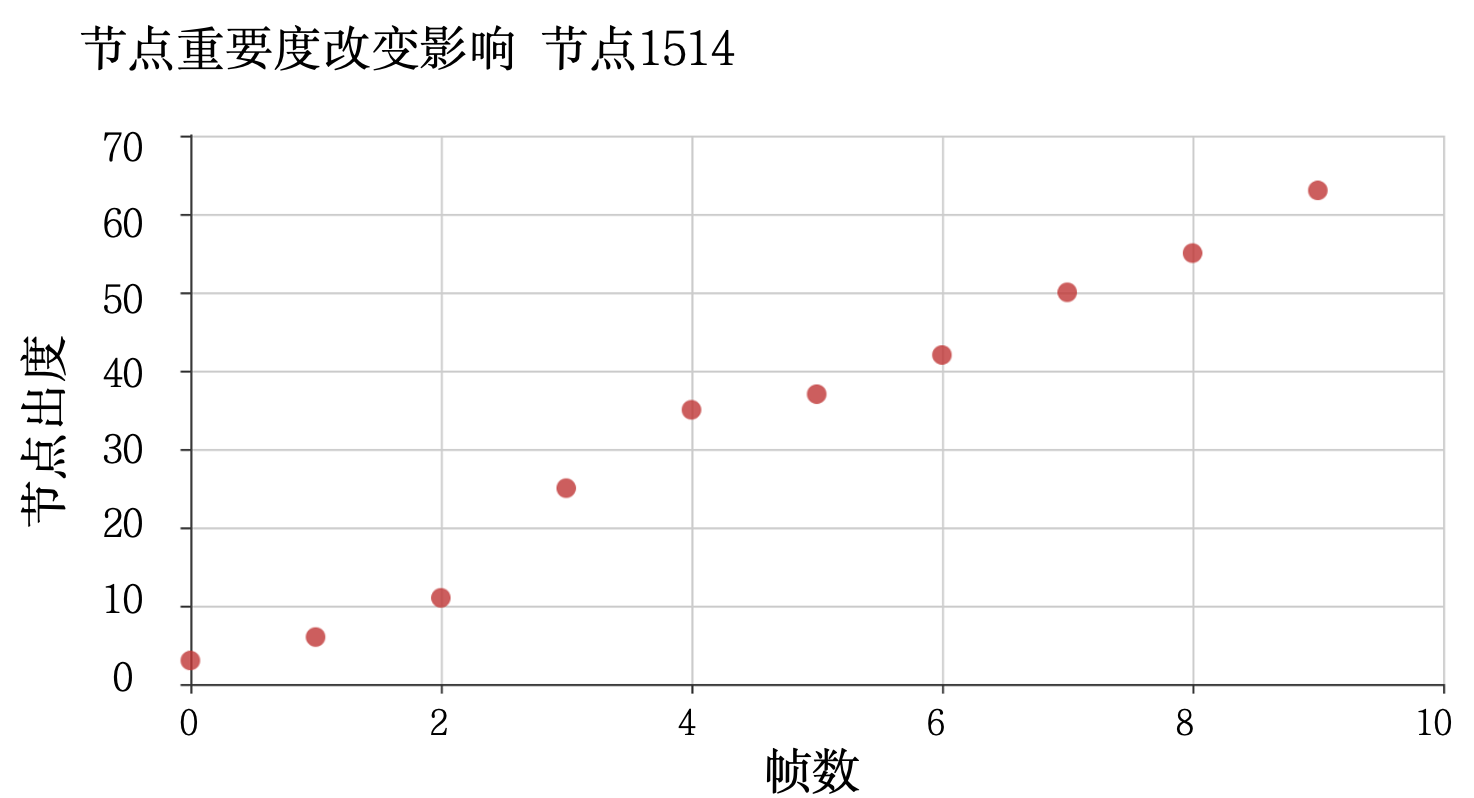
\includegraphics[scale=0.6]{important_eg1.png}
  \caption{节点重要度提升—以节点1514为例}
  \label{fig:important_eg1}
\end{figure}

\begin{figure}[H]
  \centering
  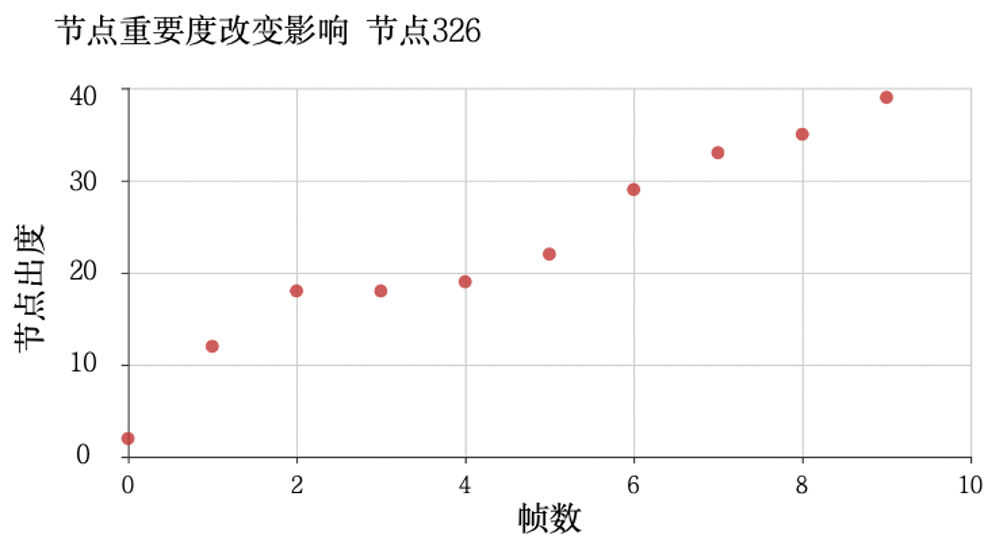
\includegraphics[scale=0.6]{important_eg2.png}
  \caption{节点重要度降低—以节点326为例}
  \label{fig:important_eg2}
\end{figure}

第5-7帧中的突发事件模拟代表着某些节点度数增长速度的临时加快。如图\ref{fig:sudden_event_eg}所示,节点1866在该事件中受到影响,第5-7帧中度数增长速度明显加快。

\begin{figure}[H]
  \centering
  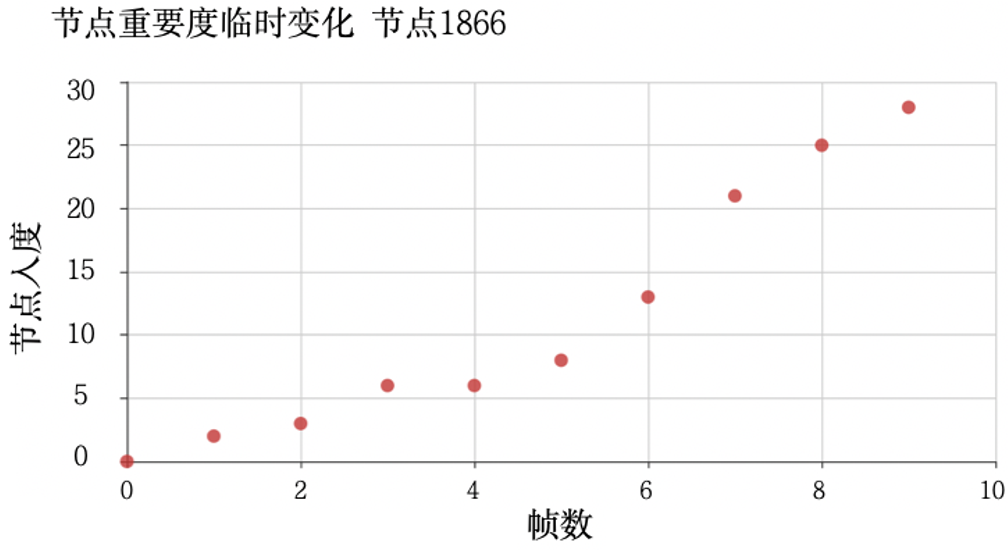
\includegraphics[scale=0.6]{sudden_event_eg.png}
  \caption{突发事件模拟—以节点1866为例}
  \label{fig:sudden_event_eg}
\end{figure}

接下来对生成结果的社区特征进行分析。此处将社区划分比例调整为$2:3:5$,并且将节点按照社区重排,结果如图\ref{fig:community_vis}所示。

\begin{figure}[H]
  \centering
  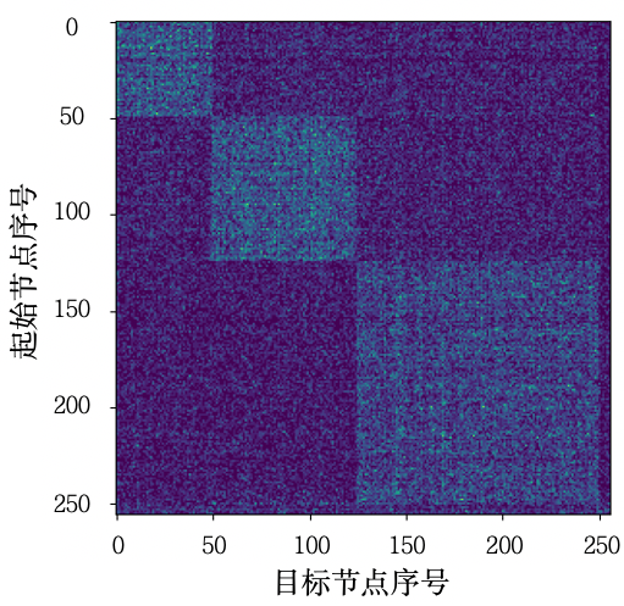
\includegraphics[scale=0.6]{community_vis.png}
  \caption{社区可视化}
  \label{fig:community_vis}
\end{figure}

我们可以清楚地看出其中的社区,这可以说明生成算法的结果符合给定的社区分布。

\section{性能分析}

此节旨在用不同的节点数、边数、帧数等配置信息进行生成,比较所用时间,用以验证生成算法的性能。

若无特殊说明,实验中共用的配置如下:

\begin{itemize}
  \item 定义了标签为student的节点、标签为friend的边,不存在多重边
  \item 出度分布采用$\lambda=2$、最大度数为100、最小度数可变的Power-Law分布
  \item 入度分布与出度分布定义方式相同
  \item 社区按照$8:2$的比例进行划分,社区参数$\rho=0.5$
  \item 不设置事件
  \item 使用ADJ格式进行存储
  \item 节点总数、分布的最小度数、边总数\footnote{边的实际数量由边生成过程中通过给定的出度分布确定}、帧数信息会分别在每个实验中说明
\end{itemize}

\subsection{所用时间随图规模的变化}

本节通过对节点数目、分布的最小度数这两项配置信息的修改,观察所用时间与图的整体规模的关系。实验中配置与结果如表\ref{tab:exp}所示。

\begin{table}[htb]
  \centering
  \caption[实验-所用时间随图规模的变化]{所用时间随图规模的变化}
  \label{tab:exp}
  \begin{minipage}[t]{0.8\textwidth}
    \begin{tabularx}{\linewidth}{lllll}
      \toprule[1.5pt]
      {\heiti 节点总数} & {\heiti 最小度数} & {\heiti 边总数} & {\heiti 帧数} & {\heiti 时间(s)} \\
      \midrule[1pt]
      100 & 3 & 867 & 10 & 0.114\\\hline
      100 & 30 & 5251 & 10 & 0.226\\\hline
      1000 & 3 & 9581 & 10 & 0.640\\\hline
      1000 & 30 & 51554 & 10 & 1.650\\\hline
      5000 & 3 & 47861 & 10 & 3.355\\\hline
      5000 & 30 & 254777 & 10 & 9.619\\\hline
      5000 & 90 & 499767 & 10 & 11.648\\\hline
      10000 & 3 & 93037 & 10 & 6.425\\\hline
      10000 & 30 & 515136 & 10 & 16.006\\\hline
      10000 & 90 & 947884 & 10 & 21.712\\\hline
      50000 & 3 & 476961 & 10 & 32.299\\\hline
      50000 & 30 & 2555196 & 10 & 81.717\\\hline
      50000 & 90 & 4736425 & 10 & 118.890\\\hline
      100000 & 3 & 953490 & 10 & 80.333\\\hline
      100000 & 30 & 5106549 & 10 & 190.093\\\hline
      100000 & 90 & 9475146 & 10 & 240.551\\
      \bottomrule[1.5pt]
    \end{tabularx}
  \end{minipage}
\end{table}

\begin{figure}[H]
  \centering
  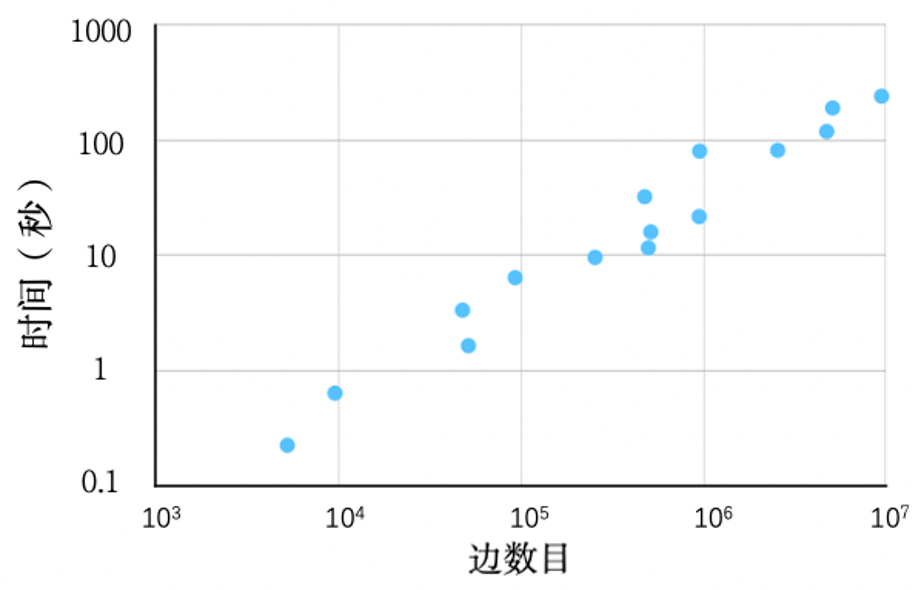
\includegraphics[scale=0.5]{edges_time.png}
  \caption{用时与边数目的关系}
  \label{fig:edges_time}
\end{figure}

将表中边数目与所用时间两项抽取出来,如图\ref{fig:edges_time}所示,可以看出总体时间的增长随边数目呈线性关系。

\subsection{所用时间随帧数的变化}

本节将节点数目、分布的最小度数固定,观察所用时间与总帧数的关系。

本实验的配置与结果如表\ref{tab:exp2}所示。

\begin{table}[htb]
  \centering
  \caption[实验-所用时间随帧数的变化]{所用时间随帧数的变化}
  \label{tab:exp2}
  \begin{minipage}[t]{0.8\textwidth}
    \begin{tabularx}{\linewidth}{lllll}
      \toprule[1.5pt]
      {\heiti 节点总数} & {\heiti 最小度数} & {\heiti 边总数} & {\heiti 帧数} & {\heiti 时间(s)} \\
      \midrule[1pt]
      10000 & 30 & 509966 & 1 & 3.096\\\hline
      10000 & 30 & 508252 & 3 & 7.663\\\hline
      10000 & 30 & 512508 & 9 & 14.937\\\hline
      10000 & 30 & 512150 & 27 & 37.837\\
      \bottomrule[1.5pt]
    \end{tabularx}
  \end{minipage}
\end{table}

\begin{figure}[H]
  \centering
  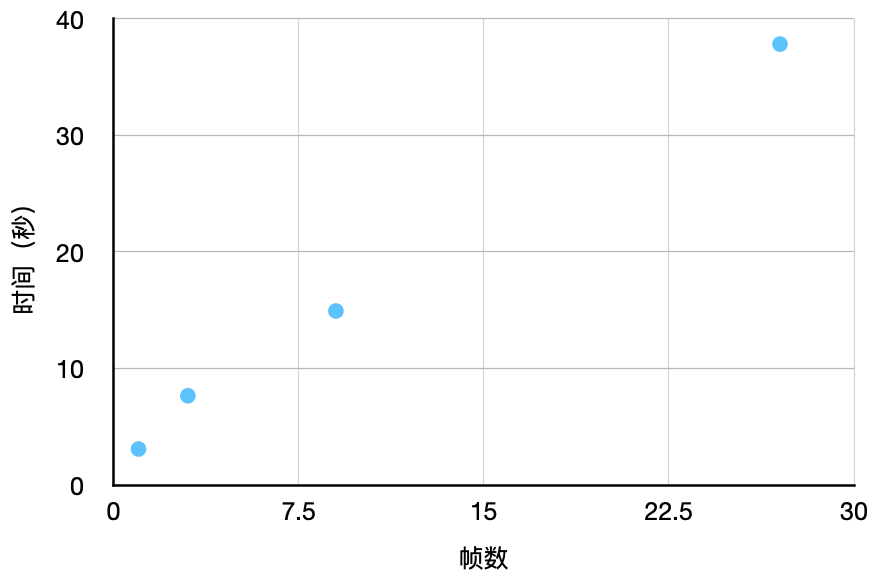
\includegraphics[scale=0.5]{time_stampnum.png}
  \caption{用时与帧数的关系}
  \label{fig:stamps_time}
\end{figure}

将表中帧数与所用时间两项抽取出来,如图\ref{fig:stamps_time}所示。从表\ref{tab:exp2}和图\ref{fig:stamps_time}中可以看出,所用时间与总帧数有着很大的关联,总耗时随着总帧数增加逐渐增长,速度略慢于线性关系。

更大的总帧数会导致每帧中的保存工作消耗更多的时间,并且总的循环次数增多会导致单次循环产生的边更少,生成效率更低。
% !TeX root = ../main.tex

\chapter{结论}
\label{cha:chapter99}

本文使用事件巧妙地定义了一些典型的社交网络图结构的时序动态性,用一些结构特征的变化来模拟真实社交网络中的变化特性,是一个新颖的动态社交网络图定义方式。这一定义方法高度抽象化,聚焦于图结构本身的特征,并非完全使用模拟的方式进行动态的定义,因此可以方便、快速地通过这种定义进行动态图的生成。

基于对动态图的认识与研究,本文在已有的静态社交网络图快速生成方法\cite{FastSGG}基础上进行了改进和扩展,提出并实现了一个动态图的配置与生成算法,并且构建了一个完整的动态社交网络图生成系统。

在本文设计与实现的动态图生成算法中,设计并应用了节点映射(NodeMap)的概念,将许多动态图事件的实现关联到这一结构中,从而顺利进行动态图的事件执行。

% 同时,文中进行了大量的优化方面的尝试,成功提速了动态图的生成工作,节省了效率。

本文实现的系统中使用前后端架构,利用Vue.js、Echarts、ElementUI进行前端配置、可视化展示体系的搭建,利用Django进行后端资源、任务的管理,并使用多线程技术进行生成过程的管理,有效提升了系统的可用性、易用性。与原始的JSON形式的配置方式相比,文中提供的动态图生成管理系统可以更高效、更方便地进行动态图的配置、运行、结果查看与可视化,并且可以方便用户进行远程生成与管理。

% 在这次课题的研究过程中,笔者对动态图的特性以及社交网络的一些特征有了更深入的理解,此次项目也锻炼了笔者的前后端技术应用水平和软件工程开发水平,较全面地提升了笔者的专业素养。

本次研究主要遇到的问题就是如何定义与实现动态社交网络图的动态性同时便于生成、如何基于图的邻接表用随机方式进行高效生成而非直接使用模拟的方式。为了解决这些问题,本文关注一些社交网络本身的结构特征信息,包括图中节点度数的分布规律、社区结构、节点重要性的相对排序,通过名为节点映射这一结构的使用,将节点按照其度数大小进行排序组织,让节点蕴含的度数特性在节点映射中得以保存,并且将相关事件的处理通过对节点映射的修改来实现。

除此之外,在动态图管理生成系统的搭建过程中也曾经遇到一些问题,如怎样实现数据项的动态添加、如何更高效地进行图的可视化、如何避免耗时较长的生成过程阻塞后端服务进程等。为了解决前端配置与可视化展示的相关问题,本文中使用了流行的Vue.js框架与ECharts框架进行数据的绑定与可视化,用ElementUI进行界面的美化操作。为了解决后端阻塞的问题,文中使用多线程的方式进行处理,收到生成请求之后在后台开启一个新的线程,线程结束后将结果反馈给主线程以便用户进行结果的查看、分析。

由于时间与经验所限,本课题中提出的用事件进行定义、用节点映射进行实现的方法并不是尽善尽美。这样的方式使用的是图结构的相关特征,关注点在于动态图的结构方面变化,而一定程度上忽视了结构变化内在的联系与规律,如真实网络中一些节点的变化趋势并非相同,符合某些特征的节点更有可能在给定的事件中受到影响,因此数据生成、事件处理方面使用的随机方式有很大的提升空间。并且本次研究中使用了高度自由化的配置方法,可能使得用户在所提供的可配置选项中进行的配置不一定符合真实网络中的相关特征,一些动态图的内部节点间的关联特征难以用这里提出的基于随机的动态图模拟方法进行模拟。

对动态社交网络图生成方面的研究还有很大的空间,在对真实网络进行更多分析的基础上也许能提出更合适的方法。结合神经网络的方式,用RNN提取之前的节点特征来进行后续事件配置,指导事件中影响到的节点的选择与具体的事件执行过程,可能会有更符合真实情况的结果。


% 其它部分
\backmatter

%% 本科生要求的几个索引。
\listoffigures    % 插图索引
\listoftables     % 表格索引
\listofequations  % 公式索引

% 参考文献
% \bibliographystyle{thuthesis-numeric}      % 顺序编码制
% \bibliographystyle{thuthesis-author-year}  % 著者-出版年制
\bibliographystyle{thuthesis-bachelor}     % 本科生参考文献的著录格式
\bibliography{ref/refs}

% % 致谢
% % !TeX root = ../main.tex

\begin{acknowledgements}
  这篇工作的完成要感谢我的导师王朝坤副教授对本人的精心指导,感谢王彬彬学长和顾天凯学长的帮助与指点!
\end{acknowledgements}


% % 声明
% \statement

% % 附录
% \appendix
% % !TeX root = ../main.tex

\begin{survey}
\label{cha:survey}

\title{Survey on Graph Generation}
\maketitle

Graphic data that includes nodes and edges shows everywhere in our life.
For example, friendship between people and interactions on social
networks, citation of papers, and activities like transferring accounts
in the financial field can be modeled with graphs. Using graphs to do
analysis and research is popular, so graph data plays an important role
and is the basis of this field.

Graphic data generation is an important issue, and synthetic datasets
are widely used in research. When we find an algorithm, we need to do
experiments on different scales and different types of datasets.
Usually, it is not enough to use real datasets only. On the one hand,
the number of public datasets is small. On the other hand, the size of a
dataset is decided by its data, we can find it difficult to get
extremely large scale real-world social graphs. So we need to generate
new data or expand from the existing data to obtain data that we needed,
usually of the same distribution and different sizes. Therefore,
synthetic datasets are a good choice for researchers.

Among the generating methods for synthesizing datasets, there are
rule-based methods for graph generation, and there are also some
algorithms for graph generation based on a given graph's pattern.

There are two points to consider: the similarity between synthetic
datasets and real data, and the efficiency of the generation method.
Over the past decades, many researchers have focused on the problem and
have made in-depth research based on the characteristics of real graphs.
It includes some traditional methods based on distribution and
probability theory, and there are also some methods based on neural
networks.

Most of the generation methods are for static graphs, but generation of
dynamic graphs has also been studied by some researchers. Dynamic graphs
can be seen as the time series of graphs, so they're more difficult to
generate.

\section{Traditional Methods}

These methods are based on the priori structural assumptions from the
observation of social networks, such as power law, small-world property,
the community structure of social networks. We can use pieces of
knowledge from probability theory and some result of distribution from
the real-world to generate nodes, edges as well as attributes. In these
methods, some optimization steps are introduced to speed up the process
of generation.

Here are two of this kind of method, S3G2 and FastSGG.

\subsection{S3G2\cite{Minh2012S3G2}}

“S3G2” is short for “Scalable Structure-correlated Social Graph
Generator”, it is a generator that can produce scalable a social network
graph which is structure-correlated. So-called “structure-correlated” is
not the attributes of a single node or the community-structure we
usually talk about, it mainly focuses on the way nodes happen to be
connected, which is the edges of the graph based on the nodes'
attributes or labels.

It's a novel graph generator that can take node attribute similarity
into account when generating edges of a graph. It can keep similar graph
connectivity features known in real social networks, which can be an
important factor in the performance of graph algorithms so that it can
produce graphs suitable for the testing process of many graph
algorithms.

It also has the ability to scale up in parallel, allowing large-scale
results to be generated quickly on clusters.

\subsubsection{Method Ideas}

In a social network, the distribution and characteristics of nodes and
edges in a graph are related to previously generated nodes, edges, and
the attributes of them. For example, people from different countries
have different names. Another example is that people who attend the same
university at the same time are more likely to become friends.
Therefore, it is necessary to consider node attributes and their
associated distribution for graph generation, but other graph generators
did not consider this before this paper was published.

The generation period of S3G2 is divided into several stages, each of
which revolves around a correlation dimension. A method called MapReduce
is also used to reduce disk I/O pressure so that it can generate larger
data graphs.

In the algorithm, the attribute information of the nodes needs to be
assigned, and the probability of edges between the two nodes can be
derived from their attributes.

\subsubsection{Formal Definition}

Class and dictionary information is introduced in the graph generated by
S3G2, so this graph is different from the concept of the graph we
usually define. In this graph, besides representing the relationship
between two instances through edges, an instance has certain attributes
in the form of edges. So there are two kinds of edges, one of them shows
the connection of objects, the other points the object to its attribute
info; there are also two kinds of nodes, one of them is an object and
the other is the attribute value.

Formally, the graph is represented as \(G(V, E, P, C)\). Where:

\begin{itemize}
\item
  \(C\) denotes a collection of classes;
\item
  \(V\) denotes a node, possibly a text or an instance of a class,
  \(V=L \cup \bigcup_{c \in C} O^{c}\), where \(L\)denotes a collection
  of all text, \(O^c\)denotes an instance belonging to category \(C\);
\item
  \(P\) denotes attributes,
  \(P=\left\{P^{L(x)} | \forall x \in C\right\} \cup\left\{P^{E(x, y)} | \forall x, y \in C\right\}\),
  where \(P^{L(x)}\) denotes the set of text attributes for the category
  \(x\), and \(P^{E(x,y)}\) denotes the set of attributes from category
  \(x\)to the edge of the category \(y\);
\item
  \(E\) denotes an edge, denoted by a tuple of three,
  \(E=\left\{\left(n_{1}, n_{2}, p\right) | n_{1} \in O^{x} \wedge\left(\left(n_{2} \in L \wedge p \in P^{L(x)}\right) \vee\left(n_{2} \in O^{y} \wedge p \in P^{E(x, y)}\right)\right)\right\}\),
  which can indicate that an instance has some attribute, or that there
  is a relationship between two instances and the attributes of that
  relationship are given. There are the following two cases:
\item
  \(n_1\) (an instance of the class \(x\)) has an attribute named \(p\)
  which is \(n_2\);
\item
  There is a relationship between \(n_1\) (it's an instance of the class
  \(x\)) and \(n_2\) (it's an instance of the class \(y\)), it has the
  attribute \(p\).
\end{itemize}

\vspace{0.2cm}

S3G2 also introduced the concept of a dictionary for each attribute
\(l\in P^{L(x)}\), specifying structure \(PD_l(D, R, F)\) for a
dictionary that has a corresponding attribute \(l\). Here \(D\) denotes
a dictionary, \(R\) for a sorting function, \(F\) for a probability
density function, these are defined as follows:

\begin{itemize}
\item
  Here the dictionary \(D\) is a set of length \(|D|\),
  \(D=\{v_1,., v_{|D|}\}\);
\item
  \(R\) is a bijection from \(D\) to \(\{1,.,|D|\}\), which gives each
  value in the dictionary order. (To save storage space, S3G2 actually
  set an order threshold of \(N\), where the top-N values in the
  dictionary are stored, but the rest of the values are assigned a
  random order);
\item
  \(F\) is a probability density function, which takes an order
  \(\{1,.,|D|\}\) to \([0,1]\) and gives the probability for each order.
  The cumulative distribution function \(F'=\sum\limits_{i=1}^r F(i)\)
  is also introduced in this paper.
\end{itemize}

\vspace{0.2cm}

Because different attribute parameters can lead to different results, we
need to put this information in the above functions. For example,
\(R[z](c)\) denotes the sorted value of \(c\) based on the attribute
\(z\).

\subsubsection{Algorithm for Probability of Edges}

A simple method is to use a degree distribution of \(N(·)\) to determine
the degree of this node each time when we need to generate a new node in
a graph generation process. The distribution is typically a power-law
distribution (\(N(h)\sim \gamma \cdot h^{-\lambda}\)). Under different
attributes, \(\gamma\) and \(\lambda\) may be different, so the
attribute information can be used to determine the degree distribution
parameters of a node in S3G2.

However, the practice of only using this method can result in a smaller
graph, which usually contains isolated submaps or have tree structures
with only a few layers.

In order to generate large-scale, highly connected graphs in a better
method, we need to consider how edges are generated after a generation
action finished for a batch of nodes. Because the attributes of a node
affect how many neighbors it may have and how the nodes connect, this
computation of this can be expensive. Therefore, S3G2 simplified the
calculation by using correlation dimensions, which represent the
probability of connections between nodes with their attributes as
follows:

\begin{itemize}
\item
  Given two types of nodes, \(O^x\) and \(O^y\), the attributes of the
  edges between the two types, \(e\in P^{E(x, y)}\), we can define the
  correlation dimension, \(CD_e(M^x, M^y, F)\). Here are two similarity
  functions, \(M^x, M^y\). And \(F\) is a probability distribution
  function.
\item
  The similarity function \(M\) converts each node into a number. After
  all the nodes have been calculated, they can be sorted using these
  numbers to determine the similarity between the nodes by their
  distance calculated by the order information.
\item
  For many social network data, we consider the connection of the same
  category (e.g. people). In this condition, \(x=y\), \(M^x=M^y\).
\item
  \(F\) is a function which accepts the difference of the order between
  one node and another node, and can output the probability of
  connection between the two nodes. For more efficient calculations, the
  number of input values has an upper limit of \(W.t\), which means that
  each node only considers connecting to nodes within the distance
  \(W.t\), which is some of the most similar nodes. This upper limit,
  \(W.t, \) is called window length because it is equivalent to
  considering only the information of subsequent nodes of that length
  (within a window) each time when the program considers the node's
  adjacency.
\end{itemize}

\vspace{0.2cm}

After getting the edges between nodes between which the distance is no
more than \(W.t\) according to the relevant dimensions, we can generate
some other edges for all the nodes without considering their distance,
using a pure random probability function.

\subsubsection{MapReduce}

This is an algorithm that enables S3G2 to support parallelism:

\begin{itemize}
\item
  The map function can be run in parallel on a cluster to process input
  data and the result will be returned with an additional key;
\item
  According to the generated key, the result will be sent to different
  reducers;
\item
  The key can be used to sort the data to get the similarity between
  them;
\item
  The reduce function processes this stream of data. Similar data can be
  processed in the same reducer. Here, we will sort the correlation
  dimensions and generate the edges by using the method of the sliding
  window.
\end{itemize}

\vspace{0.2cm}

As mentioned before, when the correlation dimensions are used to process
data, the method called sliding window is used. The sliding window will
slide on the sorted nodes and generate the edges between the similar
nodes. Because only similar data is considered, it can be divided into
multiple operations on different reducers.

Because there are different attributes, MapReduce must be operated every
time in every different correlation dimensions. Another issue to
consider is the order of dependencies. Due to the dependency between
different attributes and nodes, it is necessary to consider the
dependent relationship first. For example, if we need to generate chats
or comments between friends, we need to first consider the generation of
a friend relationship, then consider the generation of comments.

\subsection{FastSGG\cite{FastSGG}}

FastSGG is a configurable social graph generator which can generate
trillion-scale social graphs efficiently. In the generation process,
social network features are taken into account. Users can specify some
characteristics of the graph, which can be flexibly adapted to many
different scenarios. The generated graphs have some known social network
characteristics, such as small-world, power-law degree distribution,
community structure, and has advantages in generation efficiency and
scalability.

An efficient Degree Distribution Generation model (\(D^2G\)) is proposed
in this paper. There are two basic steps in the process of graph
generation: determination of out-degree for a source vertex and
determination of a target vertex to construct an edge. In the \(D^2G\)
model proposed in the paper, it only takes \(O(1)\) to determine the
degree and each target vertex each time, so it is a suitable model for
large-scale map generation.

The methods presented in this paper are not limited to the power-law
distribution. For any distribution, \(D^2G\) can be used to generate
vertices if either probability density function (PDF, defined for
continuous variables) or probability mass function (PMF, defined for
discrete variables) is given.

\subsubsection{Schema Definition}

A graph is represented in the form of \(G=(V, E)\) in FastSGG. Each
vertex \(v\) in \(V\) is a tuple of three, which can be written in the
form of \((id, lbl, attr)\). Each edge \(e\) in \(E\) can be written in
the form of an edge tuple \((v_s,  v_t, lbl, attr)\). In both vertex
tuples and edge tuples, \(lbl\) denotes a label, which we can also find
in the schema definition; \(attr\) is attributes that are represented as
a set of key-value pairs.

We can define the schemas of vertices, edges, and community as follows:

\begin{itemize}
\item
  Vertex schemas are expressed in the form of
  \(VS = (lbl, amount, attr)\). This triple means we want to generate
  nodes labeled \(lbl\), the total amount of which is \(amount\) and the
  attribute information is provided in \(attr\);
\item
  Edge schemas can be expressed in the form of
  \(ES = (lbl, lbl_s, lbl_t, amount, distr_{in}, distr_{out}, attr)\),
  which indicates that we want to generate edges labeled \(lbl\), the
  total amount of which is \(amount\), which are from vertices labeled
  \(lbl_s\)and the target vertices are labeled \(lbl_t\). In-degree
  distribution of target vertices and out-degree distribution of source
  vertices are \(distr_{in}\) and \(distr_{out}\), respectively, and the
  attribute information is provided in \(attr\);
\item
  A community schema
  \(CS = (lbl_e, amount, \lambda_s, \lambda_t, \rho)\) shows that the
  community is labeled \(lbl_e\), and the total number of communities is
  \(amount\). The community size conforms to a power-law distribution,
  \(\lambda_s, \lambda_t\)denotes the power-law parameters of the
  community size in source and target vertices, respectively. \(\rho\)
  is the community fusion parameter, controls the number of edges
  between different communities. Larger \(\rho\) means that there will
  be more edges among communities.
\end{itemize}

\vspace{0.2cm}

\subsubsection{General Graph Generation}

We can use an adjacency matrix \(M\) of size \(n_s\times n_t\) to
represent the graph and \(M_{i,j}=1\) means there is an edge from
\(v_i\)to \(v_j\).

The generation process is a streaming process, each time for each node,
its output is derived from the probability distribution, and each target
vertex is determined from the distribution information so that we can
generate an edge. In the form of the matrix, we do the following things:

\begin{itemize}
\item
  For each row (each source vertex), we first determine how many 1s
  there will be by the determination of out-degree \(outd\);
\item
  Then we need to determine the target vertices. In other words, we use
  the algorithm to determine \(outd\) cells and fill in 1s.
\end{itemize}

\vspace{0.2cm}

These two steps are the edge generation process. We need to generate
random numbers that conform to a given probability distribution. Random
operations are performed here using the inverse of the cumulative
distribution function, which is \(F^{-1}\). We can generate a uniformly
distributed random number \(u\) in the range of \([0, 1]\) so that we
can use \(F^{-1}(u)\) to get a random number that conforms to the given
probability distribution.

\subsubsection{Social Graph Generation}

The significant difference between a social graph and a general graph is
that there are community structures in a social graph. Since communities
are such structures with groups of vertices densely connecting
internally and sparsely connecting externally, we can do a series of row
and column transformations on the adjacency matrix to make the vertices
of the same communities next to each other to get obvious block
structures on the main diagonal.

To generate connections between different communities, this paper uses
\(d_{out}(u)\) to express the out-degree of vertex \(u\),
\(d_{out}^i(u)\) for the out-degree of with vertices inside the same
community, and \(d_{out}^e(u) = d_{out}(u) - d_{out}^i(u)\) for the
out-degree of \(u\) with vertices in other communities. The PDF for
\(d_{out}^e(u)\) of vertex \(u\) as follows:

\[p(x)=\left\{\begin{array}{ll}
{\alpha e^{-\frac{x}{1+\rho}}} & {\text { if } x \in\left[1, outd_{\max }^{\prime}\right]} \\
{0} & {\text { otherwise }}
\end{array}\right.\]

Here \(\alpha\) is a normalization parameter such that
\(\int_{1}^{o u t d_{m a x}^{\prime}} \alpha e^{-\frac{x}{1+\rho}} \mathrm{d} x=1\),
\(\rho\) is the community fusion parameter user-defined in community
schemas and is a real number between 0 and 1.

So we can use the inverse of the cumulative distribution function
\(F^{-1}\) to take sample and get \(d_{out}^e(u)\) for vertices.
Equivalently, we can just solve the equation rather than first
calculating the function \(F^{-1}\), which is:

\begin{itemize}
\item
  For any real number \(y \in [0,1]\), we can find the best \(outd\)
  such that
  \(\int_{1}^{o u t d} \alpha e^{-\frac{x}{1+\rho}} \mathrm{d} x=y\).
\item
  We can calculate and eventually get:
  \[outd =-(1+\rho) \log \left(e^{-\frac{1}{1+\rho}}+y\left(e^{-\frac{o u t d_{\max }^{\prime}}{1+\rho}}-e^{-\frac{1}{1+\rho}}\right)\right)\]
\end{itemize}

\vspace{0.2cm}

To generate \(d_{out}\) for each vertices, we can first get a random
variable \(y\) that conforms to a uniform distribution on \([0,1]\),
then use the method above to get corresponding \(d_{out}\).

\subsubsection{Streaming Graph Generation}

To generate a graph that is continually evolving like the ones in
real-world, we need to specify how vertices and edges are generated over
time. In this paper, a parameter called growing rate (\(r_g\)) which
controls the number of new vertices and edges each generation
sub-process is introduced. \(r_g\) is in the interval \([0,1]\), the
smaller \(r_g\) is, the graph will grow slower each generation
sub-process, but the number of generation sub-processes will be bigger.

The algrithom uses \(pc_{lt}\) and \(pc_{tg}\) to control the number of
vertices each sub-process, and \(pc\) means the ratio between the number
of vertices in the current generation sub-process and that of all
vertices. If total number of vertices is n, in sub-processes,
\(pc_{lt}, pc_{tg}\) will be
\([(0, r_g), (r_g, 2r_g), (2r_g, 3r_g),...,(1-r_g, 1)]\). So before the
\(i\)th sub-process starts, we already have \(r_g \times (i-1)\) of
total vetices generated, and each sub-process we will generate \(r_g\)
of total vertices.

\subsubsection{The \(D^2 G\) Model}

In social networks, the degree distribution of vertices is usually a
discrete distribution. Theoretically, we can directly calculate and use
the inverse of the cumulative distribution function \(F^{-1}\) to
calculate the required random variable, but in order to improve
efficiency, \(D^2G\)model is proposed in this paper to only take
\(O(1)\) to determine the degree and each target vertex each time.

To generate out-degree, we first calculate CDF:

\[\alpha=\frac{1}{\sum\limits_{i=d_{\min }}^{d_{\max }} P(D=i ; \theta)}\]

\[F(x)=\sum_{i=d_{\min }}^{x} \alpha \cdot P(D=i ; \theta)\]

Here \(x\in [d_{min}, d_{max}]\).

Then we define
\(G(z)=\underset{x}{\arg \max } F(x) \leq z, x \in\left[d_{\min }, d_{\max }\right]\),
\(z\in\left\{i \cdot \text { step } | i \in N^{+}, \text {step }=\min p(x), i \cdot \text { step } \leq 1\right\}\).
So we can use \(G(\lfloor \frac y{step}\rfloor \times step)\) to get
\(F^{-1}(y)\).

To choose a target vertex, similarly to the process of generation of
out-degree, we assign each node with a in-degree with the information of
the distribution, and sort all the nodes, so that we can do cumulation
and get function \(F_s\) whose input is in-degree:

\[F_{s}(x)=\sum_{i=i n d_{m i n}}^{x} \beta \cdot i \cdot \alpha \cdot P\left(D=i ; \theta_{i n}\right)\]

\[\beta=\frac{1}{\sum_{i=i n d_{m i n}}^{i n d_{m a x}} i \cdot \alpha \cdot P\left(D=i ; \theta_{i n}\right)}\]

Compared to \(F(x)\), here we accumulated the in-degree rather than just
accumulated the probability. So if we use \(F_s^{-1}\) we can get the
in-degree of the target vertex we need.

For a random number \(y\in [0,1]\), in order to get
\(F_s(x_1) \le y \le F_s(x_2)\), there are two functions can help to
find suitable \(F_s(x_1), F_s(x_2)\):

\[H_{1}(z)=F_{s}\left(\arg \max _{x} F_{s}(x) \leq z\right)\]

\[H_{2}(z)=F_{s}\left(\arg \min _{x} F_{s}(x) \geq z\right)\]

\[x_{1}=\arg \max _{x} F_{s}(x) \leq z, x_{2}=\arg \min _{x} F_{s}(x) \geq z\]

\[z \in\left\{i \cdot \text { step } | i \in N^{+}, \text {step }=\min \left(\left\{F_{s}(x+1)-F_{s}(x) | x \in\left[i n d_{m i n}, i n d_{m a x}\right)\right\}\right), i \cdot s t e p \leq 1\right\}\]

So we can use \(H_1(y)\) and \(H_2(y)\) to get \(F_s(x_1), F_s(x_2)\).
Then we can find \(x_1, x_2\). But only use \(x_1, x_2\) we can't
determine which node, so we need to do the following things.

We define:

\[ G_{1}(z) =\sum_{i=i n d_{m i n}}^{x_{1}} i \cdot \alpha \cdot P\left(D=i ; \theta_{i n}\right)\]

\[ G_{2}(z) =\sum_{i=i n d_{m i n}}^{x_{2}} i \cdot \alpha \cdot P\left(D=i ; \theta_{i n}\right) \]

So we can use \(G_1(z)\) and \(G_2(z)\) to get the range where the
target node exist.

We can think of a simple distribution between in-degree \(x_1\) and
\(x_2\). If \(y = H_1(z)\), we can use \(G_1(z)\), and if
\(y = H_2(z)\), we can use \(G_2(z)\). Since \(y \in [H_1(z), H_2(z)]\),
so we use
\(G_1(z) + \left(G_2(z) - G_1(z)\right) \times \frac {y-H_1(z)}{H_2(z)-H_1(z)}\)
to get target vertex ID.

So we can find that after we have finished the preparations, the
determination the degree and each target vertex each time has time
complexity of \(O(1)\).

Based on this method, I will do some research in the field of dynamic
social graph generation.

\section{Methods Based on Neural Network}

A key open challenge in the area of graph generation is developing
methods that can directly learn generative models from an observed set
of graphs. There are some works based on neural network to learn
directly from data which can improve the fidelity of generated graphs.
By way of contrast, some of traditional methods based on a priori
structural assumptions usually can't keep some structure properties such
as communities.

Here are some approaches to generate graphs based on neural network:

\begin{itemize}
\item
  Flatten the adjacency matrix into a vector: Some methods use
  vector-representation to use generative models such as VAE or GAN. The
  adjacency matrix a graph is flattened into a vector of length \(n^2\).
  These approaches cannot naturally generalize to graphs of varying
  size, and requires training on all possible node permutations or
  specifying a canonical permutation, both of which require \(O(n!)\)
  time in general.
\item
  Use node-embedding result: First use node-embedding methods
  to encode nodes into a vectors, then calculate edge probablilities
  based on pairwise relationships between learned node embeddings. This
  kind of approches is only well-defined when given a fixed-set of
  nodes, and is limited to learning from a single input graph rather a
  set of graphs.
\item
  Use RNN to remember the graph generated so far: Use RNN to
  generate graphs, so that the hidden state can hold information of the
  nodes or edges that are already generated. So we can use these
  information to guide the following generation steps.
\end{itemize}

\vspace{0.2cm}

\subsection{GraphRNN\cite{You2018GraphRNN}}

GraphRNN is a deep autoregressive model. GraphRNN learns to generate
graphs by training on a representative set of graphs and decomposes the
graph generation process into a sequence of node and edge formations,
conditioned on the graph structure generated so far. GraphRNN can
generate diverse graphs that match the structural characteristics of a
target set.

GraphRNN can be viewed as a hierarchical model, where a graph-level RNN
maintains the state of the graph and generates new nodes, while an
edge-level RNN generates the edges for each newly generated node. Here
nodes don't have attributes so the generation of nodes is easy.

To solve some problems faced in the area of graph generation, GraphRNN
uses the following methods:

\begin{itemize}
\item
  To solve the problem of the fixed and small size of the generated
  graph generated by some methods, GraphRNN models a graph in an
  autoregressive (or recurrent) manner. This manner can be seen as a
  sequence of additions of new nodes and edges and it is able to capture
  the complex joint probability of all nodes and edges in the graph. So
  GraphRNN can generate graphs of different sizes.
\item
  Graphs have non-unique representations which makes \(n!\) equivalent
  adjacency matrices for a single graph. To solve this problem, a
  breadth-first-search (BFS) node-ordering scheme is introduced.
  GraphRNN can represent some adjacency matrices into the same BFS tree.
  And the tree-structure induced by BFS allows us to limit the number of
  edge predictions made for each node during training.
\item
  Edge formation in graphs involves complex structural dependencies. The
  method GraphRNN use RNN to store structures that have already
  genereated to influence the following generation steps.
\item
  Some methods can only use a single graph to get the generation model,
  but we can train GraphRNN with several graphs so that we can generate
  graphs based on a set of graphs.
\end{itemize}

\vspace{0.2cm}

\subsubsection{Definition of Notations}

In the paper, the auther use \(\pi\) to denote a node permutation while
use \(\Pi\) to denote the set of all \(n!\) possible node permutations.
\(A^\pi\) which is a matrix of shape \(n\times n\) is the adjacency
matrix under the node permutation \(\pi\), while
\(A^{\Pi}=\{A^\pi|\pi \in \Pi \}\) is the set of adjacency matrices that
all correspod to the same underlying graph.

To learn the generation model of a graph, we need to learn
\(p_{model}(G)\) which is a distribution over graphs, based on a set of
observed graphs \(\mathbb{G}=\left\{G_{1}, \ldots, G_{s}\right\}\)
sampled from data distribution \(p(G)\), where each graph may have a
different number of nodes and edges.

For each of the graphs, we assume that we may observe any node ordering
\(\pi\) with equal probability, \emph{i.e.},
\(p(\pi) = \frac 1{n!} , \forall \pi \in \Pi\). The generative model
needs to be capable of generating graphs where each graph could have
exponentially many representations, which is distinct from previous
generative models for images, text, and time series.

% As shown in Figure \ref{survey:GraphRNN}, GraphRNN use \(S_i^\pi\) which is a vector of length \(i - 1\) to denote
As shown in Figure A-1, GraphRNN use \(S_i^\pi\) which is a vector of length \(i - 1\) to denote
the adjacency vector which records the adjacency relationship between
node \(\pi(v_i)\) and nodes
\(\left(\pi(v_1), \pi(v_2),...,\pi(v_{i-1})\right)\). We need to use
edge-level RNN to predict \(S_i^\pi\).
\(S^\pi=f_S(G,\pi)=(S_1^\pi, ..., S_n^\pi)\) is used to denote all the
adjacency relationships, and \(f_G(·)\) is used to generate the graph
based on \(S^\pi\).

\subsubsection{Modeling Graphs as Sequences}

\begin{figure}
  \centering
  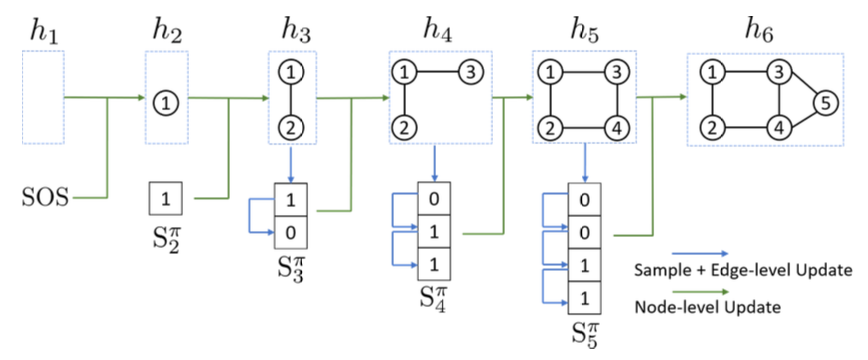
\includegraphics[scale=0.5]{graphrnn_sequences.png}
  \caption*{Figure A-1  Adjacency Vector in GraphRNN}
  \label{survey:GraphRNN}
\end{figure}

GraphRNN is based on the generation of nodes and edges, key point of
which is the estimation of \(p(S^\pi)\). Due to the sequential nature of
\(S^\pi\), we further decompose \(p(S^\pi)\) as the product of
conditional distributions over the elements:
\(p(S^\pi)=\prod\limits_{i=1}^{n+1}p(S_i^\pi|S_1^\pi, ...,S_{i-1}^\pi)\).

There are two funcitons in the calculation, a \emph{state-transition}
function \(f_{trans}\) and an \emph{output} function \(f_{out}\):

\begin{itemize}
\item
  \(f_{trans}\) is used to calculate hidden state \(h_i\) based on the
  previous hidden state and the adjacency vector,
  \(h_i=f_{trans}(h_{i-1}, S_{i-1}^\pi)\). \(h_i\in \R^d\) is a vector
  that encodes the state of the graph generated so far.
\item
  \(f_{out}\) is used to get the distribution of \(S_i^\pi\).
  \(\theta_i=f_{out}(h_i)\), \(S_i^\pi \sim \mathcal{P}_{\theta_{i}}\).
\end{itemize}

\vspace{0.2cm}

In general, \(f_{trans}\) and \(f_{out}\) can be arbitrary neural
networks, and \(\mathcal{P}_{\theta_{i}}\) can be an arbitrary
distribution over binary vectors.

\subsubsection{BFS Node-Ordering}

We can arrange the nodes to get a more effective method. So we can use
\(S^{\pi}=f_{S}(G, \operatorname{BFS}(G, \pi))\) rather than
\(S^{\pi}=f_{S}(G, \pi)\).

\(\operatorname{BFS}(G, \pi)\) means that we take a random permutation
\(\pi\) as input, picks \(π(v_1)\) as the starting node and appends the
neighbors of a node into the BFS queue in the order defined by \(\pi\).

Since the BFS function is many-to-one, \emph{i.e.}, multiple
permutations can map to the same ordering after applying the BFS
function.

There are two essential benefits:

\begin{itemize}
\item
  We only need to train on all possible BFS orderings, rather than all
  possible \(n!\) node permutations, \emph{i.e.}, multiple node
  permutations map to the same BFS ordering, providing a reduction in
  the overall number of sequences we need to consider.
\item
  The BFS ordering makes learning easier by reducing the number of edge
  predictions we need to make in the edge-level RNN; in particular, when
  we are adding a new node under a BFS ordering, the only possible edges
  for this new node are those connecting to nodes that are in the
  “frontier” of the BFS (\emph{i.e.}, nodes that are still in the BFS
  queue). In other words, if we find
  \((v_i, v_{j-1})\in E, (v_i, v_{j})\notin E, i < j \le n\), we can say
  that there are no edges between \(v_{\le i}\) and \(v_{>j}\).
\end{itemize}

\vspace{0.2cm}

\section{Dynamic Network Generation}

As far as I know, there are not such methods that can generate a dynamic
network to simulate some emergencies in the real-world. Most of the
existing methods are to split the process of graph generation into
several steps, but this will result in a series of graphs that follow
the same distribution and cannot be able to show the characteristics of
evolution.

For example, in FastSGG we can divide the generation of a single graph
into several sub-processes so that only some of the vertices are
generated in each sub-process. In most of the other methods, we can also
do such a thing to get a series of graphs.

There are also some dynamic graph generation methods based on behavior.
For example, Bob de Caux and others published a paper in 2013 \cite{De2014Dynamic}, which is based on
agent interaction behavior. The details are as follows:

\subsection{Dynamic, small-world social network generation through
local agent interactions\cite{De2014Dynamic}}

The basic idea of the model is that a network is created by collisions
between \textbf{agents} that are in “social space”. This way of
creating networks can represent many social interactions, such as
real-world person-to-person meetings and on-line meetings though social
media.

The structure of a social network can be controlled by altering
parameters of the agent's movement, such as the distance it can travel.

\subsubsection{Introduction to the Model}

So-called “social space” is a 2-dimensional space and the Euclidean
distance between any two objects will represent a social distance.

Numer of agents is fixed and agent particles are distributed randomly,
with each agent representing a potential node in the social network. The
starting point for each agent will be defined initially as the home
position and represents the point to which the agent will return after a
journey. A random angle of travel and a random range will be assigned to
each of the agents, and the range is get from a function
\(\text{agent range} =-\ln \left(\frac{x}{\lambda\left(1+\mu w_{s}\right)}\right), x\in [0,1]\).
\(w_s\) means the number of direct contacts or “neighbors”,
\(\lambda, \mu\) are fixed parameters and \(x\) is the random number
chosen to generate a range for an agent. So that we can get the target
point of the agent using the angle and the range.

From a social network viewpoint, we can view this as each agent
occupying a fixed base within the social space, from which it can
interact with others. In the model, there is a factor that the
probability of founding a connection with someone nearby in the social
space is much greater than for someone further away.

There are three stages of the movement:

\begin{itemize}
\item
  Outward movement: the agent will move to the target at a constant
  velocity. And after get there, it will reassign its target.
\item
  Homeward movement: the agent will move to its home position at a
  constant velocity. And after get there, it will reassign its target.
\item
  Post-collision movement: after colliding with another agent, the agent
  will adjust its home position. Then it will get a new target.
\end{itemize}

\vspace{0.2cm}

So-called “collision” means that two agents pass within a radius width
of each other. This will lead to the formation of the two agent nodes.

Home position of an agent \(r\) will be changed according to the
formula:
\(h_{r}^{\text {new }}=h_{r}+\boldsymbol{v}_{\boldsymbol{r s}}\left(\frac{\alpha}{\beta w_{r}+1}\right)\).
Here \(\boldsymbol{v}_{\boldsymbol{r s}}\) is the vector from \(h_r\) to
\(h_s\); \(h_r, h_s\) are the original home of the two agents of the
collision; and \(w_r\) is the number of neighbors of \(r\).
\(\alpha, \beta\) are the parameters of the system which can be seen as
a “gravity” factor. \(\beta\) is multiplied to the number of neighbors
so that it can be seen as the “local” gravity and \(\alpha\) as a
“global” gravity.

\section{Conclusion}

% These methods are from different perspectives, I have extracted the key
% ideas of the generation of them into Figures \ref{survey:Brief1} and \ref{survey:Brief2}.

These methods are from different perspectives, I have extracted the key
ideas of the generation of them into Figures A-2 and A-3.

\begin{figure}
  \label{survey:Brief1}
  \centering
  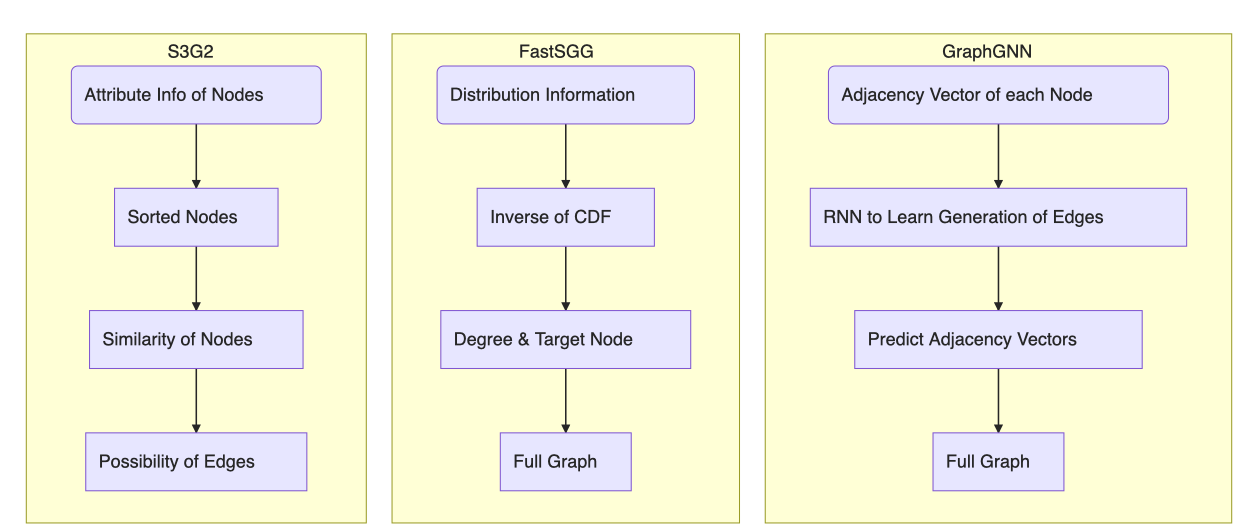
\includegraphics[scale=0.7]{image-20200514153223238.png}
  \caption*{Figure A-2  Key Ideas of S3G2, FastSGG and GraphGNN}
\end{figure}

\begin{figure}
  \label{survey:Brief2}
  \centering
  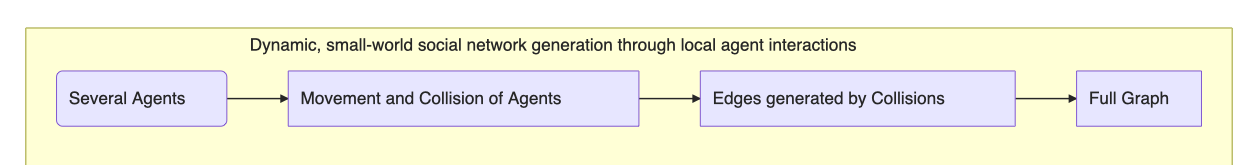
\includegraphics[scale=0.7]{image-20200514153223215.png}
  \caption*{Figure A-3  Key Idea of De2014Dynamic}
\end{figure}

I will do some research in dynamic social graph generation based on
FastSGG. Users of the generator can decide the changes over time, and
they will be able to simulate many different situations.


\bibliographystyle{plainnat}
\bibliography{ref/refs,ref/appendix}

\end{survey}
       % 本科生:外文资料的调研阅读报告
% % \input{data/appendix-translation}  % 本科生:外文资料的书面翻译
% % \input{data/appendix}

% % 个人简历
% % !TeX root = ../main.tex

\begin{resume}

  \resumeitem{个人简历}

  1997 年 5 月 2 日出生于 山西 省 阳泉 市。

  2016 年 8 月考入 清华 大学 软件学院软件工程专业。

  % \researchitem{发表的学术论文} % 发表的和录用的合在一起

  % % 1. 已经刊载的学术论文(本人是第一作者,或者导师为第一作者本人是第二作者)
  % \begin{publications}
  %   \item Yang Y, Ren T L, Zhang L T, et al. Miniature microphone with silicon-
  %     based ferroelectric thin films. Integrated Ferroelectrics, 2003,
  %     52:229-235. (SCI 收录, 检索号:758FZ.)
  %   \item 杨轶, 张宁欣, 任天令, 等. 硅基铁电微声学器件中薄膜残余应力的研究. 中国机
  %     械工程, 2005, 16(14):1289-1291. (EI 收录, 检索号:0534931 2907.)
  %   \item 杨轶, 张宁欣, 任天令, 等. 集成铁电器件中的关键工艺研究. 仪器仪表学报,
  %     2003, 24(S4):192-193. (EI 源刊.)
  % \end{publications}

  % % 2. 尚未刊载,但已经接到正式录用函的学术论文(本人为第一作者,或者
  % %    导师为第一作者本人是第二作者)。
  % \begin{publications}[before=\publicationskip,after=\publicationskip]
  %   \item Yang Y, Ren T L, Zhu Y P, et al. PMUTs for handwriting recognition. In
  %     press. (已被 Integrated Ferroelectrics 录用. SCI 源刊.)
  % \end{publications}

  % % 3. 其他学术论文。可列出除上述两种情况以外的其他学术论文,但必须是
  % %    已经刊载或者收到正式录用函的论文。
  % \begin{publications}
  %   \item Wu X M, Yang Y, Cai J, et al. Measurements of ferroelectric MEMS
  %     microphones. Integrated Ferroelectrics, 2005, 69:417-429. (SCI 收录, 检索号
  %     :896KM)
  %   \item 贾泽, 杨轶, 陈兢, 等. 用于压电和电容微麦克风的体硅腐蚀相关研究. 压电与声
  %     光, 2006, 28(1):117-119. (EI 收录, 检索号:06129773469)
  %   \item 伍晓明, 杨轶, 张宁欣, 等. 基于MEMS技术的集成铁电硅微麦克风. 中国集成电路,
  %     2003, 53:59-61.
  % \end{publications}

  % \researchitem{研究成果} % 有就写,没有就删除
  % \begin{achievements}
  %   \item 任天令, 杨轶, 朱一平, 等. 硅基铁电微声学传感器畴极化区域控制和电极连接的
  %     方法: 中国, CN1602118A. (中国专利公开号)
  %   \item Ren T L, Yang Y, Zhu Y P, et al. Piezoelectric micro acoustic sensor
  %     based on ferroelectric materials: USA, No.11/215, 102. (美国发明专利申请号)
  % \end{achievements}

\end{resume}


% % 本科生的综合论文训练记录表
% \includepdf[pages=-]{scan-record.pdf}

\end{document}
